%!TEX root = skripsi.tex
%
% Template Laporan Skripsi/Thesis 
%
% @author  Andreas Febrian, Lia Sadita 
% @version 1.03
%
% Dokumen ini dibuat berdasarkan standar IEEE dalam membuat class untuk 
% LaTeX dan konfigurasi LaTeX yang digunakan Fahrurrozi Rahman ketika 
% membuat laporan skripsi. Konfigurasi yang lama telah disesuaikan dengan 
% aturan penulisan thesis yang dikeluarkan UI pada tahun 2008.
%

%
% Tipe dokumen adalah report dengan satu kolom. 
%
\documentclass[12pt, a4paper, onecolumn, oneside, final]{report}

\usepackage{arabtex}
\usepackage{utf8}
\setcode{utf8}
\usepackage{amsmath}
\usepackage{amssymb}
\usepackage{enumitem}
\usepackage{pdfpages}
\usepackage{verbatim}
\usepackage{natbib}
% Load konfigurasi LaTeX untuk tipe laporan thesis
\usepackage{uithesis}

\usepackage{subcaption}

\newcolumntype{L}[1]{>{\raggedright\let\newline\\\arraybackslash\hspace{0pt}}m{#1}}
\newcolumntype{C}[1]{>{\centering\let\newline\\\arraybackslash\hspace{0pt}}m{#1}}
\newcolumntype{R}[1]{>{\raggedleft\let\newline\\\arraybackslash\hspace{0pt}}m{#1}}
% Load konfigurasi khusus untuk laporan yang sedang dibuat
%!TEX root = skripsi.tex
%-----------------------------------------------------------------------------%
% Informasi Mengenai Dokumen
%-----------------------------------------------------------------------------%
% 
% Judul laporan. 
\var{\judul}{Pengembangan Korpus ...}
% 
% Tulis kembali judul laporan, kali ini akan diubah menjadi huruf kapital
\Var{\Judul}{Pengembangan Korpus ...}
% 
% Tulis kembali judul laporan namun dengan bahasa Ingris
\var{\judulInggris}{Building Textual Entailment Corpus using Wikipedia Revision History Data with Co-training Method}

% 
% Tipe laporan, dapat berisi Skripsi, Tugas Akhir, Thesis, atau Disertasi
\var{\type}{Skripsi}
% 
% Tulis kembali tipe laporan, kali ini akan diubah menjadi huruf kapital
\Var{\Type}{Skripsi}
% 
% Tulis nama penulis 
\var{\penulis}{Aditya Rama}
% 
% Tulis kembali nama penulis, kali ini akan diubah menjadi huruf kapital
\Var{\Penulis}{Aditya Rama}
% 
% Tulis NPM penulis
\var{\npm}{1306397854}
% 
% Tuliskan Fakultas dimana penulis berada
\Var{\Fakultas}{Ilmu Komputer}
\var{\fakultas}{Ilmu Komputer}
% 
% Tuliskan Program Studi yang diambil penulis
\Var{\Program}{Ilmu Komputer}
\var{\program}{Ilmu Komputer}
\var{\programEng}{Computer Science}
% 
% Tuliskan tahun publikasi laporan
\Var{\bulanTahun}{Januari 2017}
% 
% Tuliskan gelar yang akan diperoleh dengan menyerahkan laporan ini
\var{\gelar}{Sarjana Ilmu Komputer}
% 
% Tuliskan tanggal pengesahan laporan, waktu dimana laporan diserahkan ke 
% penguji/sekretariat
\var{\tanggalPengesahan}{13 Januari 2017}
% 
% Tuliskan tanggal keputusan sidang dikeluarkan dan penulis dinyatakan 
% lulus/tidak lulus
\var{\tanggalLulus}{03 Januari 2017}
% 
% Tuliskan pembimbing 
\var{\pembimbing}{Rahmad Mahendra, S.Kom., M.Sc.}
\var{\pembimbingdua}{}
% 
% Alias untuk memudahkan alur penulisan paa saat menulis laporan
\var{\saya}{penulis}
\var{\Saya}{Penulis}

%-----------------------------------------------------------------------------%
% Judul Setiap Bab
%-----------------------------------------------------------------------------%
% 
% Berikut ada judul-judul setiap bab. 
% Silahkan diubah sesuai dengan kebutuhan. 
% 
\Var{\kataPengantar}{Kata Pengantar}
\Var{\babSatu}{Pendahuluan}
\Var{\babDua}{Tinjauan Pustaka}
\Var{\babTiga}{Rancangan Pengembangan Korpus}
\Var{\babEmpat}{Implementasi}
\Var{\babLima}{Evaluasi dan Analisis Hasil}
\Var{\babEnam}{Penutup}

% Daftar pemenggalan suku kata dan istilah dalam LaTeX
\usepackage[bahasa]{babel}
\addto\captionsbahasa{\renewcommand\bibname{Daftar Referensi}}
\hyphenrules{bahasa}
%!TEX root = skripsi.tex
%
% Hyphenation untuk Indonesia 
%
% @author  Andreas Febrian
% @version 1.00
% 
% Tambahkan cara pemenggalan kata-kata yang salah dipenggal secara otomatis 
% oleh LaTeX. Jika kata tersebut dapat dipenggal dengan benar, maka tidak 
% perlu ditambahkan dalam berkas ini. Tanda pemenggalan kata menggunakan 
% tanda '-'; contoh:
% menarik
%   --> pemenggalan: me-na-rik
%

\hyphenation{
    % alphabhet A
    a-na-li-sa a-tur 
    a-pli-ka-si 
    % alphabhet B
    ba-ngun-an 
    be-be-ra-pa 
    ber-ge-rak
    ber-ke-lan-jut-an 
    ber-pe-nga-ruh 
    % alphabhet C
    ca-ri
    % alphabhet D
    di-ban-ding-kan
    di-de-fi-ni-si-kan
    di-ha-rap-kan
    di-ka-te-go-ri-kan
    di-mi-li-ki-nya
    di-se-rah-kan
    di-sim-pan di-pim-pin de-ngan da-e-rah di-ba-ngun da-pat di-nya-ta-kan 
    di-sim-bol-kan di-pi-lih di-li-hat de-fi-ni-si
    di-se-su-ai-kan
    % alphabhet E
    e-le-men
    e-ner-gi eks-klu-sif
    % alphabhet F
    fa-si-li-tas
    % alphabhet G
    ga-bung-an ge-rak
    % alphabhet H
    ha-lang-an
    he-te-ro-gen
    % alphabhet I
    i-ngin
    % alphabhet J
    % alphabhet K
    ke-hi-lang-an
    ku-ning 
    kua-li-tas ka-me-ra ke-mung-kin-an ke-se-pa-ham-an
    ke-te-pat-an
    kon-fi-gu-ra-si
    % alphabhet L
    ling-kung-an
    % alphabhet M
    me-min-ta
    me-mo-del-kan
    me-mo-ri
    men-de-fi-ni-si-kan
    me-neng-ah
    meng-a-tas-i me-mung-kin-kan me-nge-na-i me-ngi-rim-kan 
    meng-u-bah meng-a-dap-ta-si me-nya-ta-kan mo-di-fi-ka-si
    meng-a-tur
    meng-au-to-ma-si
    meng-a-ko-mo-da-si
    me-ngo-rek-si
    % alphabhet N
    nya-ta non-eks-klu-sif
    % alphabhet O
    % alphabhet P
    pa-ra-lel
    peng-ala-mat-an
    pen-ting
    penga-da-an
		pe-nye-rap-an 
		pe-ngon-trol
    pe-mo-del-an
    pe-ran  pe-ran-an-nya
    pe-rin-tah
    pem-ba-ngun-an pre-si-den pe-me-rin-tah prio-ri-tas peng-am-bil-an 
    peng-ga-bung-an pe-nga-was-an pe-ngem-bang-an 
    pe-nga-ruh pa-ra-lel-is-me per-hi-tung-an per-ma-sa-lah-an 
    pen-ca-ri-an peng-struk-tur-an
    pe-ner-bang-an
    pro-se-sor
    % alphabhet Q
    % alphabhet R
    ran-cang-an
    % alphabhet S
    se-dang-kan
    se-ring
    si-mu-la-si sa-ngat    
    % alphabhet T
    te-ngah
    ter-da-pat
    % alphabhet U
    u-sa-ha
    % alphabhet V
    % alphabhet W
    % alphabhet X
    % alphabhet Y
    % alphabhet Z
    % special
    MATLAB
    basmalah
    sam-ping
    hardware
    software
    voiced
    overlap
    frame
    bit
    rate
    support
    vector
    machine
    Gaussian
    mixture
    model
    dynamic
    pro-gram-ming
    auto-ma-tically
    mem-ba-ca
    teks-tual
    eks-trak-si
    di-je-las-kan
    be-nar
    sa-lah
    teks-tual
    dengan
    me-re-pre-sen-ta-si
    me-re-pre-sen-ta-si-kan
}
% Daftar istilah yang mungkin perlu ditandai 
%!TEX root = skripsi.tex
%
% @author  Andreas Febrian
% @version 1.00
% 
% Mendaftar seluruh istilah yang mungkin akan perlu dijadikan 
% italic atau bold pada setiap kemunculannya dalam dokumen. 
% 

\var{\license}{\f{Creative Common License 1.0 Generic}}
\var{\bslash}{$\setminus$}
\var{\ioa}{\f{input}}
\var{\iob}{\f{output}}
\var{\br}{\f{bit rate}}
\var{\fr}{\f{frame}}
\var{\quran}{Al-Qur'an}

%\usepackage[backend=bibtex]{biblatex}
%\addbibresource{bib.bib}

% Awal bagian penulisan laporan
\begin{document}
\lefthyphenmin=5
\righthyphenmin=7
%
% Sampul Laporan
%!TEX root = skripsi.tex
%
% Sampul Laporan

%
% @author  unknown
% @version 1.01
% @edit by Andreas Febrian
%

\begin{titlepage}
    \begin{center}    
        \begin{figure}
            \begin{center}
                
\includegraphics[width=2.5cm]{pics/makara.png}
            \end{center}
        \end{figure}    
        \vspace*{0cm}
        \bo{
        	UNIVERSITAS INDONESIA\\
        }
        
        \vspace*{1.0cm}
        % judul thesis harus dalam 14pt Times New Roman
        \bo{\Judul} \\[1.0cm]

        \vspace*{2.5 cm}    
        % harus dalam 14pt Times New Roman
        \bo{\Type}

        \vspace*{3 cm}       
        % penulis dan npm
        \bo{\Penulis} \\
        \bo{\npm} \\

        \vspace*{5.0cm}

        % informasi mengenai fakultas dan program studi
        \bo{
        	FAKULTAS \Fakultas\\
        	PROGRAM STUDI \Program \\
        	DEPOK \\
        	\bulanTahun
        }
    \end{center}
\end{titlepage}


%
% Gunakan penomeran romawi
\pagenumbering{roman}

%
% load halaman judul dalam
\addChapter{HALAMAN JUDUL}
%!TEX root = skripsi.tex
%
% Halaman Judul Laporan 
%
% @author  unknown
% @version 1.01
% @edit by Andreas Febrian
%

\begin{titlepage}
    \begin{center}\begin{figure}
            \begin{center}
                
\includegraphics[width=2.5cm]{pics/makara.png}
            \end{center}
        \end{figure}    
        \vspace*{0cm}
        \bo{
        	UNIVERSITAS INDONESIA\\
        }
        
        \vspace*{1.0cm}
        % judul thesis harus dalam 14pt Times New Roman
        \bo{\Judul} \\[1.0cm]

        \vspace*{2.5 cm}    
        % harus dalam 14pt Times New Roman
        \bo{\Type} \\
        % keterangan prasyarat
        \bo{Diajukan sebagai salah satu syarat untuk memperoleh gelar \\
        \gelar}\\

        \vspace*{3 cm}       
        % penulis dan npm
        \bo{\Penulis} \\
        \bo{\npm} \\

        \vspace*{5.0cm}

        % informasi mengenai fakultas dan program studi
        \bo{
        	FAKULTAS \Fakultas\\
        	PROGRAM STUDI \Program \\
        	DEPOK \\
        	\bulanTahun
        }
    \end{center}
\end{titlepage}

%
% setelah bagian ini, halaman dihitung sebagai halaman ke 2
\setcounter{page}{2}

% sementara ga usah
% load halaman pengesahan
%\addChapter{LEMBAR PERSETUJUAN}
%%!TEX root = skripsi.tex
%
% Halaman Pengesahan
%
% @author  Andreas Febrian
% @author  Ardhi Putra Pratama
% @version 1.1
%

\chapter*{HALAMAN PERSETUJUAN}

\vspace*{0.2cm}
\noindent 

\noindent
\begin{tabular}{l l p{11cm}}
	\bo{Judul}&: & \judul \\ 
	\bo{Nama}&: & \penulis \\
	\bo{NPM}&: & \npm \\
\end{tabular} \\

\vspace*{1.2cm}


\noindent\begin{minipage}[b]{0.6\hsize}
  \raggedright
  Laporan \type~ini telah diperiksa dan disetujui.\\[0.3cm]
  
  \tanggalPengesahan \\[2cm]
  
  \underline{\pembimbing}\\[0.1cm]
  Pembimbing \type
\end{minipage}
\hfill
\begin{minipage}[b]{0.4\hsize}
  \raggedleft
  .\\[2cm]
  \underline{\pembimbingdua}\\[0.1cm]
  Pembimbing \type
\end{minipage}

\newpage
%
% load halaman orisinalitas 
\addChapter{LEMBAR PERNYATAAN ORISINALITAS}
%!TEX root = skripsi.tex
%
% Halaman Orisinalitas
%
% @author  Andreas Febrian
% @version 1.01
%

\chapter*{\uppercase{halaman pernyataan orisinalitas}}
\vspace*{2cm}

\begin{center}
	\bo{\type~ini adalah hasil karya saya sendiri, \\ 
	dan semua sumber baik yang dikutip maupun dirujuk \\
	telah saya nyatakan dengan benar.} \\
	\vspace*{2.6cm}
	
	\begin{tabular}{l c l}
	\bo{Nama} & : & \bo{\penulis} \\
	\bo{NPM} & : & \bo{\npm} \\ 
	\bo{Tanda Tangan} & : & \\
	& & \\
	& & \\
	\bo{Tanggal} & : & \bo{\tanggalPengesahan} \\	
	\end{tabular}
\end{center}

\newpage
%
%
\addChapter{LEMBAR PENGESAHAN}
%!TEX root = skripsi.tex
%
% Halaman Pengesahan Sidang
%
% @author  Andreas Febrian, Andre Tampubolon 
% @version 1.02
%

\chapter*{HALAMAN PENGESAHAN}

\vspace*{0.4cm}
\noindent 

\noindent
\begin{tabular}{ll p{9cm}}
	\type~ini diajukan oleh&: & \\
	Nama&: & \penulis \\
	NPM&: & \npm \\
	Program Studi&: & \program \\
	Judul \type&: & \judul \\
\end{tabular} \\

\vspace*{1.0cm}

\noindent \bo{Telah berhasil dipertahankan di hadapan Dewan Penguji 
dan diterima sebagai bagian persyaratan yang diperlukan untuk 
memperoleh gelar \gelar~pada Program Studi \program, Fakultas 
\fakultas, Universitas Indonesia.}\\[0.2cm]

\begin{center}
	\bo{DEWAN PENGUJI}
\end{center}

\vspace*{0.3cm}

\begin{tabular}{l l l l }
	& & & \\
	Pembimbing&: & \pembimbing & (\hspace*{3.0cm}) \\
	& & & \\
	Pembimbing&: & \pembimbingdua & (\hspace*{3.0cm}) \\
	& & & \\
	Penguji 1&: & Alfan Farizki Wicaksono S.T., M.Sc. & (\hspace*{3.0cm})\\
	& & & \\
	Penguji 2&: & Bayu Anggorojati, S.T., M.Sc., Ph.D.  & (\hspace*{3.0cm}) \\
\end{tabular}\\

\vspace*{2.0cm}

\begin{tabular}{ll l}
	Ditetapkan di&: & Depok\\
	Tanggal&: & \tanggalLulus \\
\end{tabular}


\newpage
%
%
\addChapter{\kataPengantar}
%!TEX root = skripsi.tex
%-----------------------------------------------------------------------------%
\chapter*{\kataPengantar}
%-----------------------------------------------------------------------------%

Alhamdulillahirobbil alamin, puji dan syukur \saya~ucapkan kepada Allah SWT atas segala rahmat yang telah diberikan, sehingga laporan tugas akhir ini dapat diselesaikan pada waktunya. Tak lupa \saya~sanjungkan shalawat serta salam kepada junjungan besar, Nabi Muhammad SAW. Penulis menyadari bahwa laporan ini dapat diselesaikan berkat dukungan beberapa pihak. Oleh karena itu, \saya~ingin mengucapkan terima kasih kepada :

\begin{enumerate}
	\item Kedua Orang Tua \saya
	\item Kakak dan adik-adik \saya
	\item Nadiarani
	\item Item 4
	
\end{enumerate}
\vspace*{0.1cm}
\begin{flushright}
	Depok, Desember 2016\\[0.1cm]
	\vspace*{1cm}
	\penulis
	
\end{flushright}
%
%
\addChapter{LEMBAR PERSETUJUAN PUBLIKASI ILMIAH}
%!TEX root = skripsi.tex
% 
% @author  Andre Tampubolon, Andreas Febrian
% @version 1.01
% 

\chapter*{\uppercase{Halaman Pernyataan Persetujuan Publikasi Tugas Akhir untuk Kepentingan Akademis}}

\vspace*{0.2cm}
\noindent 
Sebagai sivitas akademik Universitas Indonesia, saya yang bertanda 
tangan di bawah ini:
\vspace*{0.4cm}


\begin{tabular}{p{4.2cm} l p{6cm}}
	\bo{Nama} & : & \penulis \\ 	
	\bo{NPM} & : & \npm \\
	\bo{Program Studi} & : & \program\\	
	\bo{Fakultas} & : & \fakultas\\
	\bo{Jenis Karya} & : & \type \\
\end{tabular}

\vspace*{0.6cm}
\noindent demi pengembangan ilmu pengetahuan, menyetujui untuk memberikan 
kepada Universitas Indonesia \bo{Hak Bebas Royalti Noneksklusif 
(Non-exclusive Royalty Free Right)} atas karya ilmiah saya yang berjudul:
\begin{center}
	\judul
\end{center}
beserta perangkat yang ada (jika diperlukan). Dengan Hak Bebas Royalti 
Noneksklusif ini Universitas Indonesia berhak menyimpan, 
mengalihmedia/formatkan, mengelola dalam bentuk pangkalan data 
(\f{database}), merawat, dan memublikasikan tugas akhir saya selama 
tetap mencantumkan nama saya sebagai penulis/pencipta dan sebagai 
pemilik Hak Cipta. \\

\noindent Demikian pernyatan ini saya buat dengan sebenarnya.

\begin{center}
	\vspace*{0.8cm}
	\begin{tabular}{lll}
		Dibuat di&: & Depok \\
		Pada tanggal&: & \tanggalPengesahan \\
	\end{tabular}\\

	\vspace*{0.2cm}
	Yang menyatakan \\
	\vspace*{2cm}
	(\penulis)
\end{center}

\newpage


%
% 
\singlespacing
\addChapter{ABSTRAK}
%!TEX root = skripsi.tex
%
% Halaman Abstrak
%
% @author  Andreas Febrian
% @version 1.00
%

\chapter*{Abstrak}

\vspace*{0.2cm}

\noindent \begin{tabular}{l l p{10cm}}
	Nama&: & \penulis \\
	Program Studi&: & \program \\
	Judul&: & \judul \\
\end{tabular} \\ 

\vspace*{0.5cm}

\noindent
\textit{Cross Lingual Word Sense Disambiguation (CLWSD)} merupakan salah satu pendekatan untuk menyelesaikan permasalahan disambiguasi makna kata di bidang NLP. Pendekatan ini memanfaatkan sebuah konsep dimana suatu kata dapat diterjemahkan menjadi beberapa kata yang berbeda tergantung dengan konteks dimana kata tersebut muncul. Keterbatasan data berupa \textit{sense tagged corpus} menjadi salah satu permasalahan yang menghambat penelitian WSD di bahasa Indonesia ini. Pada penelitian kali ini, pendekatan CLWSD akan digunakan untuk \textit{transfer sense} dari \textit{sense tagged corpus} bahasa Inggris ke bahasa Indonesia dengan memanfaatkan korpus paralel dwibahasa. Hasil dari penelitian ini merupakan \textit{sense tagged corpus} dalam bahasa Indonesia yang kemudian juga akan dicoba dalam sistem WSD yang dibuat sendiri. Pada penelitian ini, \textit{sense transfering} berhasil menghasilkan \textit{sense tagged corpus} dalam bahasa Indonesia. Selain \textit{sense tagged corpus} tersebut, sistem WSD yang dibangun juga memiliki performa diatas baseline pembanding pada \textit{target word} dan fitur tertentu yang diberikan.


\vspace*{0.2cm}

\noindent Kata Kunci: \\ 
\noindent Cross Lingual, Word Sense Disambiguation

\newpage
%
%
%!TEX root = skripsi.tex
%
% Halaman Abstract
%
% @author  Andreas Febrian
% @version 1.00
%

\chapter*{ABSTRACT}

\vspace*{0.2cm}

\noindent \begin{tabular}{l l p{11.0cm}}
	Name&: & \penulis \\
	Program&: & \programEng \\
	Title&: & \judulInggris \\
\end{tabular} \\ 

\vspace*{0.5cm}

\noindent 
Cross Language Word Sense Disambiguation (\textit{CLSWD}) is one among the methods in solving word sense disambiguation problem in NLP field. This approach utilize a concept that a word can translated to many words depend on where that word appear. Limitation in data (\textit{sense tagged corpus} in Indonesian language) become one problem that hold the development of research in Indonesian WSD. In this research, we will try using CLWSD to transfer sense from english sense tagged corpus into Indonesian by using parallel corpora. Result of this research is a sense tagged corpus in Indonesian language that will be tested by our implemented WSD system. Based on the result of the experiment, we could see that the corpus from the sense transfering process produce many data with sufficient quality. Beside the sense tagged corpora, WSD system that will be built also has a performance above the baseline on some given target words.
\vspace*{0.2cm}

\noindent Keywords: \\ 
\noindent Cross Language, Word Sense Disambiguation

\newpage

%
% Daftar isi, gambar, dan tabel
%
\tableofcontents
\clearpage
\listoffigures
\clearpage
\listoftables
\clearpage
\lstlistoflistings
\clearpage

%
% Gunakan penomeran Arab (1, 2, 3, ...) setelah bagian ini.
%
\pagenumbering{arabic}

%
%
%
\onehalfspacing
%!TEX root = skripsi.tex
%-----------------------------------------------------------------------------%
\chapter{\babSatu}
%-----------------------------------------------------------------------------%
Bab ini membahas mengenai latar belakang penelitian, perumusan masalah, tujuan dan manfaat penelitian, ruang lingkup penelitian, metodologi penelitian, serta sistematika penulisan.

%-----------------------------------------------------------------------------%
\section{Latar Belakang}
%-----------------------------------------------------------------------------%	

\textit{Word Sense Disambiguation} (WSD) merupakan salah satu tugas untuk menentukan makna terbaik dari sebuah kata. Sebuah kata sendiri dapat memiliki beberapa makna dan bergantung pada konteks dimana kata tersebut muncul. Penentuan makna kata yang paling tepat ini secara tidak langsung dapat membantu beberapa \textit{task} \textit{Natural Language Processing} ataupun \textit{Information Retrieval} lainnya seperti misalnya \textit{machine translation}. Pendekatan yang biasa digunakan untuk menyelesaikan permasalahan WSD ini pada umumnya adalah pendekatan \textit{machine learning}


Pendekatan \textit{supervised machine learning} yang dapat digunakan untuk membangun sistem WSD membutuhkan data yang tidak sedikit. Data yang dibutuhkan untuk sistem ini dapat berupa \textit{sense-tagged corpus} dimana isinya adalah kata-kata yang sudah mempunyai kelas makna kata yang tepat. Kebutuhan akan data yang relatif besar tersebut merupakan kendala yang ada pada bahasa-bahasa tertentu. Bahasa Inggris sebagai salah satu bahasa internasional mempunyai data yang cukup banyak untuk membangun sistem dengan \textit{supervised learning}. Namun demikian, bahasa Indonesia sendiri termasuk dalam \textit{under resource language} dimana data yang dapat dimanfaatkan untuk sistem WSD masih terbatas. Belum adanya data seperti \textit{sense-tagged corpus} untuk membangun sistem WSD bahasa Indonesia merupakan salah satu permasalahan yang dihadapi jika dibandingkan dengan bahasa Inggris.

Makna kata yang diberikan oleh sistem WSD pada kata-kata pada umumnya berasal dari definisi pada Wordnet. Namun demikian, membangun Wordnet secara manual untuk memenuhi kebutuhannya sebagai inventaris makna kata membutuhkan waktu dan dana yang relatif tidak sedikit. Terdapat beberapa Wordnet bahasa Indonesia yang dapat digunakan, diantaranya adalah Wordnet Bahasa (bahasa.cs.ui.ac.id) dan Wordnet Bahasa yang berasal dari proyek Nanyang Technological University (NTU).  Wordnet dari Bahasa Fasilkom UI masih memiliki sedikit \textit{sets of synonyms} (synsets) yang mana berarti banyak kata-kata yang tidak tersedia di dalamnya. Wordnet bahasa dari proyek NTU sendiri masih mengandung makna kata yang tidak sesuai. Oleh karena masalah tersebut, pada penelitian ini Wordnet yang digunakan adalah Wordnet bahasa Inggris buatan Princeton yang sudah sering digunakan untuk \textit{event} Semantic Evaluation atau Sense Evaluation. Penggunaan makna kata dari Wordnet bahasa Inggris tersebut nantinya akan dipindahkan ke kata dalam bahasa Indonesia yang bersesuaian dengan memanfaatkan sifat paralel dari korpus identik.

Pendekatan \textit{cross language} dengan bahasa Inggris sebagai pasangan korpus diharapkan dapat memperkaya \textit{resource}(data) yang masih kurang pada bahasa Indonesia. 
%-----------------------------------------------------------------------------%
\section{Perumusan Masalah}
%-----------------------------------------------------------------------------%
Beberapa pertanyaan yang menjadi rumusan masalah dalam penelitian ini yaitu:
\begin{enumerate}
	\item Bagaimana cara membangun \textit{sense tagged corpus} Bahasa Indonesia dengan pendekatan \textit{cross lingual} dari paralel korpus?
	\item Seberapa baik performa WSD dari \textit{sense tagged corpus} pada tahap pertama?
\end{enumerate}

%-----------------------------------------------------------------------------%
\section{Tujuan dan Manfaat Penelitian}
%-----------------------------------------------------------------------------%
Tujuan dari penelitian yang dilakukan adalah menghasilkan \textit{sense tagged corpus} dalam bahasa Indonesia sebagai data makna kata, dan menghitung seberapa baik performa \textit{wsd system} bahasa Indonesia yang dibuat.

%-----------------------------------------------------------------------------%
\section{Ruang Lingkup Penelitian}
Penelitian berfokus pada pemindahan \textit{sense} dari korpus paralel berbahasa Inggris ke Indonesia, dan melakukan \textit{WSD task} pada hasil pemindahan makna kata tersebut.

\textit{Word sense disambiguation} yang dilakukan pada penelitian ini hanya pada tingkatan \textit{coarse-grained} \textit{wsd}.

%-----------------------------------------------------------------------------%
\section{Metodologi Penelitian}
%-----------------------------------------------------------------------------%
Ada lima tahapan yang dilakukan pada penelitian ini. Penjelasan dari tiap tahapan adalah sebagai berikut.
\begin{enumerate}
	\item Studi Literatur \\
	Tahap ini berfokus pada pencarian informasi mengenai \textit{WSD system} baik secara umum maupun teknik yang digunakan, dan juga \textit{task} lain yang berkaitan dengan \textit{WSD} seperti \textit{word sense induction} (\textit{WSI}).
	\item Perumusan Masalah \\
	Masalah-masalah yang ada dalam penelitian nantinya dianalisis penyelesaiannya pada tahap ini.
	\item Rancangan Penelitian\\
	Proses yang melibatkan seluruh penelitian untuk menyelesaikan permasalahan yang ada.
	\item Implementasi\\
	Tahap ini merupakan implementasi dari rancangan yang sudah dibuat untuk memecahkan permasalahan yang ada.
	\item Analisis dan Kesimpulan \\
	Hasil percobaan dianalisis untuk mendapatkan gambaran seberapa baik performa dari sistem yang dibuat.
\end{enumerate}


%-----------------------------------------------------------------------------%
\section{Sistematika Penulisan}
%-----------------------------------------------------------------------------%
Sistematika penulisan yang ada dalam laporan penelitian ini sebagai berikut:
\begin{itemize}
	
	\item Bab 1 \babSatu \\
	Bab ini akan menjelaskan mengenai latar belakang, perumusan masalah, tujuan penelitian, tahapan penelitian, ruang lingkup, metodologi, dan sistematika penulisan dari penelitian ini.
	
	\item Bab 2 \babDua \\
	Bab ini akan menjelaskan mengenai konsep dan teori yang relevan dari hasil studi literatur yang telah dilakukan. Teori-teori yang dijelaskan meliputi \textit{Word sense disambiguation}, \textit{Word sense induction}, dan beberapa hal lain yang dibutuhkan pada penelitian.
	
	\item Bab 3 \babTiga \\
	Bab ini akan membahas perihal rancangan dari proses penelitian yang meliputi \textit{sense tagging} korpus Inggris, \textit{word alignment} Indonesia-Inggris, \textit{sense transfering}, dan sistem WSD bahasa Indonesia.
	
	\item Bab 4 \babEmpat \\
	Pada bab ini akan menjelaskan mengenai implementasi dari rancangan sistem yang dibuat.
	
	\item Bab 5 \babLima \\
	Pada bab ini, dijelaskan mengenai hasil penelitian beserta evaluasi dan analisisnya. 
	
	\item Bab 6 \babEnam \\
	Kesimpulan dan saran dari hasil dan pelaksanaan penelitian akan dijelaskan pada bab ini.
	
\end{itemize}
%!TEX root = skripsi.tex
%-----------------------------------------------------------------------------%
\chapter{\babDua}
%-----------------------------------------------------------------------------%
Bab ini membahas mengenai studi literatur yang digunakan selama penelitian. Studi literatur ini menjelaskan tentang hal-hal mendasar yang dibutuhkan dalam penelitian.
%-----------------------------------------------------------------------------%

\section{Semantik Leksikal}

Kata dalam suatu bahasa memiliki banyak fitur atau informasi yang terkandung di dalamnya. Informasi pada kata tersebut meliputi contoh-contoh seperti ortografi, POS Tag, dan juga makna kata. Informasi yang ada tersebut dapat dipergunakan sebagai fitur untuk merepresentasikan suatu kata.

\subsection{Fitur Kata}
Terdapat berbagai macam fitur yang dapat diambil dari informasi sebuah kata. Informasi ini meliputi bentuk-bentuk variasi kata, kelas kata, makna kata, dan lain-lain. Ortografi, sebagai salah satu fitur kata meliputi permasalahan dalam suatu kata pada bahasa mengenai ejaan, kapitalisasi, pemenggalan kata, dan lain-lain. Pada bentuk kata (morfologi), Lemma merupakan bentuk kata "dasar" seperti misalnya "\textit{run}", \textit{"ran"}, dan "\textit{runs}" memiliki lemma yang sama yaitu "run". POS Tag atau Part of Speech Tag merupakan "kategori" dari suatu kata yang didefinisikan untuk membedakan kelas-kelas yang ada seperti misalnya \textit{proper noun} (nama orang, organisasi, nama tempat, dan lain-lain), \textit{verb} (kata kerja), \textit{adjective} (kata sifat seperti "marah", "senang", dan lain-lain), \textit{adverbial}, dan semacamnya. \textit{Tool} yang digunakan untuk melakukan POS Tagging pada penelitian ini adalah \textit{tool} dari Stanford. Makna kata menyimpan informasi dari arti sebuah kata, dan satu kata bisa memiliki lebih dari satu makna. Selain informasi dalam suatu kata, terdapat relasi antara satu kata dengan kata lain seperti misalnya sinonim, homonim, polisemi, dan lain-lain. Berdasarkan informasi \citep{sheeba2013unsupervised}, sinonim merupakan relasi pada kata-kata yang berbeda namun memiliki makna yang serupa, dan homonim merupakan kata dengan ejaan atau penulisan yang sama namun memiliki makna yang berbeda. Mirip dengan homonim, polisemi merupakan suatu kata yang memiliki makna lebih dari satu. Contoh dari relasi sinonim adalah antara kata "bohong" dengan "dusta", "perspektif" dengan "sudut pandang", dan kata-kata dengan makna mirip lainnya. Contoh dari kata polisemi adalah pada kata "darah" dalam kalimat "Tangan Ani mengeluarkan darah setelah tertusuk jarum" dengan "Ani baru menyadari bahwa dia dan Rina memiliki hubungan darah". Relasi homonim antar kata dapat dilihat misalnya pada kata "rapat" yang dapat berarti "pertemuan" ataupun juga "berdekatan", sebenarnya kata ini merupakan dua buah kata yang berbeda(sehingga maknanya berbeda) hanya saja penulisan dan pengejaannya sama.

Terdapat beberapa cara untuk merepresentasikan sebuah kata sebagai fitur. Salah satu cara yang sederhana adalah dengan merepresentasikan kata sebagai \textit{one hot vector}. Pada model ini, setiap kata di dalam sebuah korpus diberikan nomor indeks untuk membangun vektor yang mewakili keberadaan kata tersebut. Jika terdapat sebuah kata yang muncul pada konteks yang ingin direpresentasikan, indeks vektor yang sama dengan indeks kata tersebut akan bernilai 1. Bila terdapat sebuah korpus dengan jumlah kata unik berjumlah 4 dengan kata-kata "Ani", "marah", "kemarin", dan "malam" (sebuah vektor dengan pangjang empat). Representasi \textit{one hot vector} untuk kalimat "Ani marah" dapat ditulis dengan vektor [1,1,0,0].

Representasi \textit{one hot vector} akan mempunyai panjang vektor yang besar jika korpus mempunyai jumlah kata unik yang besar. Terdapat bentuk representasi lain untuk membentuk vektor dari kata, salah satunya adalah dengan \textit{word embedding}. \textit{Word Embedding} menggunakan representasi bilangan \textit{real} pada vektor untuk merepresentasikan sebuah kata berdasarkan hasil \textit{training} dengan suatu korpus. Contoh representasi dari \textit{word embedding} pada suatu kata "makan" adalah vektor [0.6, -0.3, ..., 0.5] (misalnya). Vektor dari hasil \textit{word embedding} mempunyai karakteristik di mana jarak antara dua buah vektor dari kata yang mirip secara semantik bernilai kecil(dekat). Bila misalkan pada data \textit{training} untuk \textit{word embedding} terdapat banyak kalimat-kalimat berbentuk "... makan Y ..." di mana Y adalah sebuah objek berupa makanan. Maka kata-kata yang mewakili Y seperti misalnya "burger", "apel", "steak", dan lain-lain, akan memiliki vektor yang mirip dan secara implisit dapat saling menggantikan untuk menempati posisi Y tersebut. Berdasarkan keterdekatan vektor tersebut, \textit{word embedding} mampu untuk menangkap semantik dari kata-kata yang ada pada korpus.

Salah satu model \textit{word embedding} yang dapat digunakan adalah Word2Vec \citep{mikolov2013distributed}. Pada penelitian ini Word2Vec akan digunakan untuk memanfaatkan vektor \textit{word embedding} sebagai salah satu fitur percobaan skenario yang ada. 

\subsection{Wordnet}

Wordnet merupakan \textit{online lexical database} yang didesain dan untuk digunakan suatu program \citep{miller1995wordnet}. Salah satu Wordnet untuk bahasa Inggris yang sudah berkembang dan digunakan dalam berbagai penelitian adalah Wordnet yang dikembangkan Princeton (PWN atau Princeton Wordnet). Selain Wordnet bahasa Inggris, terdapat juga Wordnet Bahasa Indonesia yaitu Wordnet bahasa Indonesia dari Fakultas Komputer Universitas Indonesia (Wordnet UI) , dan Wordnet hasil penelitian pembuatan Wordnet Bahasa \citep{noor2011creating} (Wordnet Bahasa). Pada Wordnet UI terdapat sebanyak 1.203 synset, 1.659 kata unik, dan 2.261 relasi di dalamnya. Sementara itu, Wordnet Bahasa memiliki 49.668 synset, 145.696 \textit{senses}, dan 64.431 kata unik. Hal ini menunjukkan bahwa Wordnet Bahasa memiliki informasi lebih banyak dari Wordnet UI, walaupun jumlah tersebut juga mencakup beberapa kata dalam bahasa Malaysia atau Melayu. Representasi yang digunakan Wordnet adalah \textit{set of synonyms} (synset) sebagai kumpulan dari kata-kata yang memiliki kemiripan makna. Selain menyimpan kata-kata, Wordnet juga menyimpan makna dari setiap kata-kata tersebut. Informasi makna kata yang ada di dalam Wordnet sering digunakan untuk sistem WSD suatu bahasa sebagai acuan (\textit{sense inventory}). Makna kata pada Wordnet disimpan dengan \textit{uniq identifier} berupa \textit{sense key} yang memiliki format "\textbf{lemma\%key}". Salah satu contoh \textit{sense key} adalah "home\%1:06:00::" yang mana memiliki makna "\textit{Housing that someone is living in}". Representasi \textit{synset} dari Wordnet beserta relasi-relasinya tersebut dapat dimanfaatkan untuk disambiguasi makna suatu kata.

%-----------------------------------------------------------------------------%
\section{Word Sense Disambiguation}
%-----------------------------------------------------------------------------%
\textit{Word Sense Disambiguation} merupakan salah satu penelitian di bidang NLP yang bertujuan untuk menentukan makna yang paling tepat dari suatu kata berdasarkan konteks kata tersebut ditemukan. Sebagaimana kata dalam suatu bahasa bisa memiliki makna lebih dari satu (polisemi), \textit{task} ini akan menentukan makna kata mana yang paling tepat. 

Penentuan makna kalimat dilakukan dengan pemberian informasi berupa kata yang menjadi \textit{target} dan konteks berupa kalimat. Contoh proses disambiguasi yang dilakukan untuk kata \textbf{cokelat}:

\begin{lstlisting}[backgroundcolor = \color{white}]
K1: Roni memakan cokelat yang diberikan ibunya
K2: Walaupun mobil cokelat itu mahal, dia sangat ingin membelinya
\end{lstlisting}


Pada kalimat pertama (K1), \textbf{cokelat} yang dimaksud memiliki makna sebagai makanan yang terbuat dari buah \textit{cokelat}. Sementara itu, Kata \textbf{cokelat} pada kalimat kedua (K2) memiliki makna yang berbeda, di mana kata tersebut merupakan satu keterangan warna. Penentuan makna yang tepat dapat dilakukan dengan bantuan informasi konteks dari kalimat di mana kata tersebut muncul. Pada K1, kata \textbf{memakan} memberikan informasi bahwa \textit{cokelat} yang dimaksud adalah objek yang bisa dimakan. Kata yang memberikan informasi pada kalimat kedua adalah kata \textbf{berwarna} yang secara eksplisit menerangkan bahwa \textbf{cokelat} yang dimaksud adalah warna. Namun demikian, konteks maupun informasi yang bisa diambil dari kalimat tidak selalu eksplisit. Pada contoh kalimat seperti "Pohon cokelat tua di belakang rumahku sangat besar", cokelat yang dimaksud bisa bermakna "buah cokelat yang sudah tua" atau "berwarna cokelat tua".

Penentuan makna kata yang tepat oleh sistem WSD ditentukan berdasarkan konteks dari kata tersebut berada. Walaupun satu kata dapat memiliki beberapa makna, terdapat kecil kemungkinan bahwa kata yang sama digunakan dalam satu \textit{discourse} (konten dari sebuah percakapan atau bahasan) untuk menyatakan makna yang berbeda sebagaimana "\textit{one sense per discourse}" \citep{gale1992one}.

Pada umumnya, sistem WSD yang dibangun dapat menggunakan pendekatan \textit{machine learning} baik itu \textit{supervised}, \textit{semi-supervised}, maupun \textit{unsupervised}. Pendekatan yang dipilih biasanya bergantung pada data maupun \textit{resource} yang dimiliki pada suatu bahasa. Jika terdapat data/\textit{resource} yang memadai, sistem dengan pendekatan \textit{supervised} biasanya dilakukan untuk mendapatkan akurasi yang optimal. Namun demikian, untuk bahasa-bahasa dengan data/\textit{resource} yang kurang memadai, pendekatan \textit{semi-supervised} atau bahkan \textit{unsupervised} dapat dimanfaatkan untuk mendapatkan makna kata secara otomatis. 

Terdapat dua buah granularitas dalam sistem WSD yaitu \textit{coarse-grain} dan \textit{fine-grain}. Coarse-grained WSD lebih berfokus pada kata-kata yang homonim. Sementara itu, fine-grained WSD menggunakan kata-kata yang bersifat polisemi seperti misalkan disambiguasi dari kata "bulan" pada "bulan langit malam" dengan "bulan September". Pada fine-grained WSD, kata-kata yang ambigu lebih banyak dari pada coarse-grained, yang mana mengakibatkan lebih sulitnya klasifikasi yang dilakukan oleh sistem untuk menentukan makna kata yang tepat.\textit{Agreement} yang dihasilkan antar anotator pada fine-grained WSD sendiri juga relatif rendah \citep{navigli2007semeval}. Pelabelan makna yang lebih detail dari fine-grained WSD dapat dilihat pada gambar berikut.

\begin{figure}
	\centering
	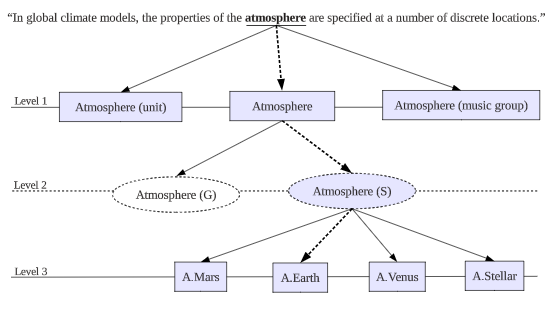
\includegraphics[width=1\linewidth]{adit_pics/coarse-fine}
	\caption{coarse dan fine-grained WSD  \citep{shen2013coarse}}
	\label{fig:coarse}
\end{figure}

Berdasarkan gambar \ref{fig:coarse}, dapat dilihat bahwa kata "\textit{atmosphere}" yang awalnya hanya dipandang sebagai 3 buah makna, dapat dipecah lagi menjadi beberapa makna yang lebih detail. Lebih banyaknya \textit{sense} yang dihasilkan mengakibatkan lebih sulitnya klasifikasi yang dilakukan dalam sistem WSD fine-grained.

Pada sistem WSD, fitur yang umum digunakan beberapa di antaranya adalah konteks kata baik dengan pendekatan Collocation dan Co-occurrence, POS Tag kata, vektor \textit{word embedding} kata. Fitur Co-occurrence lebih berfokus pada kemunculan kata pada suatu konteks baik itu dokumen, paragraf, atau kalimat. Contoh dari fitur dengan pendekatan ini adalah pada kalimat "Dia membuka halaman empat dari buku harry potter", di mana kata-kata yang ada pada kalimat tersebut dapat menjadi fitur yang menandakan keberadaan suatu kata. Pada contoh tersebut, setiap kata dapat ditandai sebagai angka 1 pada vektor 1 dan 0 jika kata tersebut muncul. Sementara Collocation lebih berfokus pada kata yang sering muncul secara bersama-sama dan kecil kemungkinannya untuk muncul bersama secara kebetulan. Jika pada contoh kalimat yang sama, fitur co-occurence hanya melihat pada kata-kata di dekat kata "halaman" (misalkan kata ini sebagai \textit{target word}), yang muncul sering dengan kata "halaman" tersebut. Pada fokus fitur ini, kata "buku" memiliki kemungkinan lebih besar untuk berada dekat dengan kata "halaman" dan kecil kemungkinan untuk muncul secara kebetulan.

\subsection{WSD Bahasa Inggris}
Terdapat berbagai penelitian yang sudah dilakukan untuk melakukan disambiguasi kata pada Bahasa Inggris. Penelitian WSD pada Bahasa Inggris sendiri lebih banyak dibandingkan dengan Bahasa Indonesia karena permasalahan WSD ini diangkat dalam beberapa \textit{event} seperti SemEval ataupun Senseval. \textit{Resource} yang digunakan sebagai \textit{sense inventory} utama pada WSD Bahasa Inggris biasanya adalah Wordnet princeton, dan beberapa data tambahan seperti misalnya Brown Corpus, SemCor, dan lain-lain. Terdapat salah satu sistem WSD yang sudah dipublikasikan dan siap digunakan untuk melakukan WSD dengan \textit{input} berupa \textit{free text} dalam Bahasa Inggris. Sistem WSD tersebut adalah "It Makes Sense" (IMS) yang dibangun oleh Zhi Zhong dan Hwee Tou Ng \citep{zhong2010makes}. Sistem  dibangun menggunakan pendekatan \textit{supervised learning} yang dapat digunakan untuk semua kata bahasa Inggris. Pada dasarnya, \textit{classifier} yang dipilih untuk \textit{task} ini adalah \textit{support vector machine} (SVM). Arsitektur yang dibangun pada IMS dapat dilihat pada gambar berikut:

\begin{figure}
	\centering
	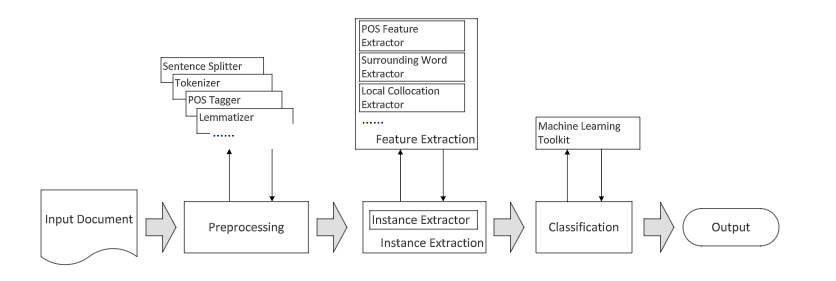
\includegraphics[width=1\linewidth]{adit_pics/Arsitektur-IMS}
	\caption{Arsitektur IMS}
	\label{fig:Arsitektur-IMS}
\end{figure}

Proses \textit{pre-processing} pada IMS dilakukan dengan empat tahapan:
\begin{enumerate}
	\item Mendeteksi batasan kalimat dengan \textit{sentence splitter}
	\item Tokenisasi dengan \textit{tokenizer}
	\item POS Tagging untuk semua token
	\item Mengubah token menjadi lemma dengan \textit{lemmatizer}
\end{enumerate}

Ekstraksi fitur dilakukan dengan mengombinasikan:

\begin{enumerate}
	\item POS Tag dari tiga buah kata di kiri dan kanan \textit{target word}, serta kata itu sendiri. 
	\item Kata-kata sekitar pada konteks kalimat ataupun kalimat tetangganya. Kata-kata yang terkandung di dalam \textit{stopwords} dan memiliki simbol atau angka dibuang dari kalimat tersebut. Kata-kata yang tersisa tersebut kemudian diubah menjadi bentuk kata dasarnya dalam huruf kecil.
	\item \textit{Local Collocation} dengan 11 buah \textit{collocation} baik itu sebelum \textit{target word} maupun setelahnya. 
\end{enumerate}

Pengujian seberapa baik performa IMS dalam melakukan  WSD \textit{task} mendapatkan hasil:

\begin{figure}
	\centering
	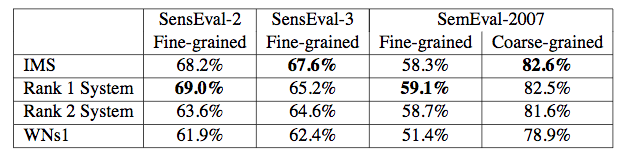
\includegraphics[width=1\linewidth]{adit_pics/Performa-IMS}
	\caption{Performa IMS \citep{zhong2010makes}}
	\label{fig:Performa-IMS}
\end{figure}

IMS digunakan pada penelitian ini karena sistem WSD ini sudah dapat digunakan untuk \textit{tagging} makna kata dengan input berupa \textit{free text}.

\subsection{WSD Bahasa Indonesia}

Terdapat dua penelitian terkait WSD Bahasa Indonesia yang ditemukan, yaitu penelitian WSD menggunakan data dari situs berita Kompas \citep{uliniansyah2006word}, dan \textit{cross lingual} WSD \citep{septiantri2013wsd}. Penelitian \citep{uliniansyah2006word} menggunakan Naive Bayes untuk klasifikasi \textit{sense} dengan fitur-fitur berupa satu kata di kiri dan kanan \textit{target}, kata kerja terdekat dari \textit{target}, konteks dokumen, dan kata kerja transitif di sekitar \textit{target word}. Sistem WSD yang dibangun tersebut memiliki hasil akurasi pada \textit{range} 73-99\%.

Pada penelitian dengan pendekatan \textit{cross lingual} WSD \citep{septiantri2013wsd}, proses diawali dengan mendapatkan makna kata dengan memanfaatkan korpus paralel dwibahasa. Proses ekstraksi makna kata tersebut akan dijelaskan pada sub-bab \textit{cross language} dalam pembahasan \textit{Word Sense Induction}. Setelah makna kata didapatkan, kata-kata yang memilki makna lebih dari satu diambil untuk dijadikan \textit{sample} untuk mengevaluasi sistem WSD yang dibangun. Setelah mendapatkan kata-kata yang ambigu, proses selanjutnya adalah mengambil fitur dari masing-masing konteks kata tersebut muncul. Ekstraksi fitur yang dilakukan adalah mengambil kata-kata yang pernah muncul pada kalimat yang mengandung \textit{target word}. Dari hasil kata-kata tersebut, vektor fitur akan direpresentasikan dengan cara yang serupa seperti \textit{bag of words} yaitu dengan vektor satu dan nol yang merepresentasikan ada tidaknya suatu kata dalam kalimat. Terdapat beberapa \textit{classifier} yang digunakan untuk dijadikan perbandingan yaitu Naive Bayes, Random Forest, dan SVM. Variasi dari seknario pada penelitian tersebut meliputi \textit{stemming}, penghilangan \textit{stopwords}, dan modifikasi korpus paralel dengan cara menggabungkan korpus Identic dengan data tambahan. Secara garis besar, akurasi yang didapatkan pada penelitian tersebut adalah ketiga buah \textit{classifier} yang dicoba dapat menghasilkan tingkat akurasi yang lebih baik dari baseline.

Penelitian \textit{cross lingual} WSD \citep{septiantri2013wsd} tersebut memiliki tujuan utama untuk mencoba pendekatan \textit{cross lingual} dalam melakukan \textit{transferring} makna kata, lalu melakukan disambiguasi terhadap makna tersebut dengan kata-kata yang sudah dipilih. Berbeda dengan penelitian tersebut, fokus dari penelitian ini adalah untuk membangun \textit{sense tagged corpus} Bahasa Indonesia dengan pendekatan yang \textit{transferring} yang mirip namun berbeda. Jika pada penelitian \citep{septiantri2013wsd} menentukan makna kata dilakukan dengan melihat \textit{sense key} yang sama (\textit{intersection}) dari kata dalam kedua bahasa, penentuan makna kata dalam penelitian ini dilakukan dengan memanfaatkan \textit{sense tagged corpus} Bahasa Inggris untuk kata-kata pada korpus Inggris, kemudian \textit{transfer} makna tersebut ke kata dalam Bahasa Indonesia yang menjadi pasangannya.
%-----------------------------------------------------------------------------%
\section{Word Sense Induction}
%-----------------------------------------------------------------------------%	
%-----------------------------------------------------------------------------%	
\textit{Word Sense Induction} (WSI) adalah sebuah \textit{task} yang mempunyai fungsi utama untuk mendapatkan makna kata dari sebuah korpus atau teks yang belum dianotasi secara otomatis. WSI dapat dilakukan jika penelitian WSD yang ingin dilakukan tidak mempunyai cukup \textit{resource} seperti misalnya Wordnet ataupun \textit{sense tagged corpus} yang \textit{reliable}. \textit{Reliable} pada hal ini dapat berarti kurangnya jumlah \textit{sense} pada data, ataupun masih sedikitnya jumlah kata-kata yang ada pada Wordnet. WSI secara tidak langsung dapat memperbanyak data yang dapat digunakan jika sistem WSD yang ingin dibangun membutuhkan data \textit{training} yang tidak sedikit. Terdapat berbagai macam pendekatan dalam melakukan \textit{sense induction}, di antaranya adalah dengan melakukan \textit{clustering} kata \citep{denkowski2009survey}, ataupun menggunakan pendekatan \textit{cross language}.
	
	\subsection{Pendekatan \textit{Clustering}}
	Dua kata dianggap dekat secara semantik jika memiliki \textit{co-occurrence} dengan kata-kata tetangganya yang sama \citep{nasiruddin2013state}. Konsep tersebut mendasari cara WSI mendapatkan \textit{sense} kata secara implisit berdasarkan hasil \textit{cluster} yang terbentuk dari data atau teks mentah (teks yang tidak dianotasi).
	
	Penarikan makna secara implisit dapat dicontohkan pada beberapa kalimat rujukan berikut \citep{denkowski2009survey}:
	
	\begin{enumerate}
		\item A bottle of tezg\"{u}no is on the table.
		\item Everyone likes tezg\"{u}no.
		\item Tezg\"{u}no makes you drunk.
		\item We make tezg\"{u}no out of corn.
	\end{enumerate}
	
	Walaupun belum terdapat informasi eksplisit makna dari tezg\"{u}no, dapat disimpulkan bahwa tezg\"{u}no mengacu pada minuman beralkohol yang memabukkan. Penarikan kesimpulan ini didapatkan dari kemunculan kata tersebut dengan kata lain pada konteks yang sama.
	
	Pada pendekatan \textit{clustering} ini, makna kata bisa didapatkan secara implisit dari hasil \textit{cluster} yang terbentuk, namun demikian pelabelan yang dilakukan untuk menentukan apa yang direpresentasikan \textit{cluster} tersebut merupakan sebuah \textit{task} tersendiri.
	
	Salah satu cara \textit{clustering} yang dijelaskan \citep{pantel2002discovering} adalah dengan mencoba beberapa algoritma seperti K-Means, Buckshot, CBC, Unicon, Bisecting K-Means, dan Average Link untuk fitur yang ditentukan. Fitur yang digunakan adalah vektor dari kata yang didapatkan dengan menghitung \textit{discounted pointwise mutual information} dari kata tersebut pada konteks kata itu muncul. Perhitungan \textit{similarity} antara dua buah kata dihitung dengan menghitung jarak vektor kedua kata tersebtu.
	
	Pada pendekatan \textit{clustering}, hasil dari \textit{cluster} yang didapat masih harus diberikan label dan makna kata tidak bisa secara eksplisit diambil dari hasil tersebut. Proses \textit{topic modeling} masih diperlukan untuk dapat menentukan "topik" apa yang menggambarkan atau merepresentasikan \textit{cluster} tersebut. 
	
	\subsection{Pendekatan \textit{Cross Language}}
	Selain pendekatan \textit{clustering}, WSI juga dapat memanfaatkan fitur di mana satu kata dari suatu bahasa, dapat diterjemahkan menjadi beberapa kata di bahasa lain. Contoh kasus tersebut dapat dilihat pada kata "halaman" berikut:

	\begin{lstlisting}[backgroundcolor = \color{white}]
	(K1-Indonesia): Aku membaca 10 halaman buku Harry Potter
	(K1-English): I read 10 pages of Harry Potter book
	(K2-Indonesia): Ani tinggal di rumah dengan halaman yang sangat luas
	(K2-English): Ani lives in a house with very large yard
	\end{lstlisting}
	
	Berdasarkan kedua pasangan kalimat tersebut, kata \textbf{halaman} dalam bahasa Indonesia dapat diterjemahkan menjadi dua buah kata dalam bahasa Inggris, yaitu \textit{page} ataupun \textit{yard}. Hal ini menunjukan bahwa terjemahan dari suatu kata bergantung pada konteks di mana kata tersebut muncul.
	
	Salah satu penelitian yang juga menggunakan pendekatan \textit{Cross-Lingual} WSI adalah penelitian \citep{septiantri2013wsd} yang memanfaatkan korpus paralel untuk menentukan makna yang tepat dari suatu kata berdasarkan makna tersebut dalam Bahasa Indonesia dan Bahasa Inggris. Proses yang digunakan untuk menentukan makna kata secara \textit{cross lingual} pada penelitian tersebut dilakukan dengan tahap-tahap:
	
	\begin{enumerate}
		\item Lakukan pemasangan kata-kata antara kedua korpus (Bahasa Inggris - Indonesia) dengan Giza++
		\item Untuk kata-kata pada setiap pasangan tersebut, berikan \textit{tag} makna kata yang mungkin dari Wordnet NTU. Contoh dari proses ini misalnya pada pasangan kata "halaman" dengan "\textit{page}". Berikan \textit{sense id} yang mungkin untuk kata "halaman" dari Wordnet NTU misalnya sense-id-1, sense-id-2, dan sense-id-3. Lakukan hal yang sama pada kata "\textit{page}", misalnya diberikan \textit{sense id} sense-id-5, sense-id-7, dan sense-id-2.
		\item Berdasarkan hasil \textit{sense id} dari proses sebelumnya, ambil \textit{sense id} yang beririsan untuk dijadikan \textit{tag} dari \textit{sense} kata tersebut. Pada contoh kata "halaman" dan "\textit{page}" tadi, maka label/\textit{tag} yang diberikan pada kata "halaman" adalah \textit{sense id} sense-id-2.
		\item Lakukan proses pelabelan \textit{tagging} makna kata tersebut untuk pasangan kata lainnya.
		\item Suatu kata yang memiliki \textit{sense id} lebih dari satu kemudian dinyatakan sebagai kata yang ambigu.
	\end{enumerate}


\section{Korpus Paralel dan \textit{Comparable}}
Terdapat dua macam korpus bilingual yang dapat dimanfaatkan untuk pemanfaatan \textit{cross language } WSD yaitu korpus paralel dan \textit{comparable}. Perbedaan utama terhadap kedua buah korpus berada pada seberapa identik kedua buah konteks yang dimilikinya. Korpus paralel memiliki kalimat dan kata-kata yang serupa antara dua buah pasangan di masing-masing korpus. Hal ini dapat dicontohkan misalnya dengan kalimat satu pada korpus bahasa Indonesia "Aku makan" dengan "I eat" pada korpus bahasa Inggris. Salah satu contoh korpus paralel adalah Catholic Bible yang dinamakan sebagai bitext \citep{rudnick2011towards} yang merupakan kitab katolik dalam bahasa yang berbeda. Berbeda dengan korpus paralel, \textit{comparable} berarti kedua kalimat atau \textit{instance} yang berpasangan hanya sebatas mirip/sama dalam suatu kategori kriteria tertentu. Dengan adanya korpus paralel dan \textit{comparable} tersebut, dibutuhkan juga alat untuk menyelaraskan (\textit{aligning}) konten pada kedua korpus tersebut. \textit{Alignment} yang dapat dilakukan memiliki beberapa tingkatan mulai dari \textit{scope} yang besar sampai kecil. \textit{Scope} besar tersebut meliputi \textit{alignment} dokumen yang mana fungsinya adalah menyelaraskan antar dokumen yang konten atau kriterianya sama. Tingkatan yang lebih kecil berikutnya yaitu kalimat di mana \textit{alignment} dilakukan pada \textit{level} kalimat (pasangan kalimat yang makna atau kriterianya sama). \textit{Alignment} dengan tingkatan yang lebih spesifik lagi adalah kata (\textit{word alignment}), di mana hasil yang didapat dari proses ini adalah pasangan kata pada kedua korpus dwibahasa yang selaras. Korpus paralel maupun \textit{comparable} ini dapat dimanfaatkan untuk sistem terkait  \textit{cross language information retrieval} (CLIR), \textit{machine translation} (MT), CLWSD, dan lain-lain.
%-----------------------------------------------------------------------------%
\section{\textit{Word Alignment}}
Tugas dari \textit{word alignment} adalah menemukan korespondensi antara kata pada teks paralel 
\citep{mihalcea2003evaluation}. Pada dasarnya, \textit{task} ini diperlukan sebagai salah satu proses dalam MT untuk mendapatkan secara otomatis kata-kata yang berpasangan dari korpus paralel dwibahasa atau lebih. Secara umum, proses dari pemasangan kata berlangsung seperti pada gambar \ref{fig:word-alignment}.

\begin{figure}
	\centering
	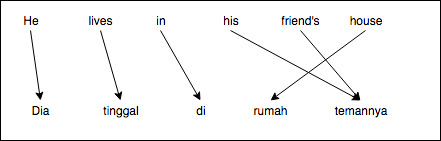
\includegraphics[width=1\linewidth]{adit_pics/wordalignment.jpeg}
	\caption{Contoh \textit{word alignment}}
	\label{fig:word-alignment}
\end{figure}

Kasus yang dapat terjadi pada proses \textit{alignment} ini salah satunya adalah ketika terdapat kata yang tidak memiliki pasangan. Contoh dari kasus tersebut dapat dilihat pada gambar \ref{fig:word-alignment-2}.

\begin{figure}
	\centering
	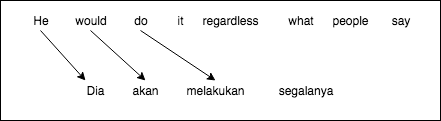
\includegraphics[width=1\linewidth]{adit_pics/contoh_word_alignment_2.png}
	\caption{Contoh lain \textit{word alignment}}
	\label{fig:word-alignment-2}
\end{figure}

Bila melihat bahasa Indonesia sebagai sumber bahasa, maka kata "segalanya" pada kalimat tersebut tidak memiliki pasangan dalam bahasa Inggris K1. Pada kasus-kasus seperti ini, biasanya akan ada token khusus yang nantinya akan berpasangan dengan kata-kata yang tidak mempunyai pasangan.

\textit{Tool} yang digunakan untuk keperluan \textit{word alignment} pada penelitian ini adalah Giza++ \citep{och03:asc}. \textit{Tool} tersebut merupakan salah satu \textit{word alignment tools} pada \textit{statistical machine translation} (SMT) yang dapat digunakan untuk memasangkan kata-kata pada dua buah korpus dwibahasa atau lebih. Terdapat beberapa \textit{word alignment tools} lain seperti Berkeley \textit{aligner}, anymalign, dan lain-lain.
%------------------------------------------- ----------------------------------%

\section{Support Vector Machine}
Salah satu \textit{classifier} yang dapat digunakan dalam \textit{supervised learning} untuk melakukan klasifikasi adalah SVM. SVM termasuk sebagai metode klasifikasi yang populer dan telah digunakan untuk berbagai permasalahan seperti klasifikasi teks, \textit{facial expression recognition}, analisis gen, \textit{word sense disambiguation}, dan lain-lain. SVM dapat dikatakan sebagai salah satu metode yang membangun aturan yang dinamakan sebagai \textit{linear classifier} yang secara teori akan menghasilkan kualitas prediksi dari \textit{unseen data} yang baik \citep{fradkin2006support}. Pada salah satu penelitian WSD Bahasa Inggris \citep{zhong2010makes}, SVM digunakan sebagai \textit{classifier} dari sistem yang dibangun.

Konsep dari cara SVM bekerja adalah dengan menemukan sebuah \textit{hyperplane} dengan \textit{margin} (jarak dari \textit{hyperplane} dengan titik kelas terdekat) yang terbesar. Pemilihan \textit{margin} dengan nilai terbesar ini ditujukan agar \textit{classifier} lebih optimal dalam memisahkan objek dengan kelas yang berbeda. Pada penelitian kali ini, SVM yang digunakan berasal dari \textit{library} Python bernama Scikit \citep{scikit-learn}.

\section{Evaluasi}

Precision, Recall, dan F-score merupakan beberapa cara perhitungan untuk merepresentasikan akurasi dari suatu sistem. Berdasarkan domain \textit{information retrieval}, precision merupakan perbandingan dari total jumlah dokumen relevan yang didapatkan oleh sistem dengan total jumlah dokumen yang didapat. Lain halnya dengan precision, recall membandingkan total dokumen relevan yang didapatkan dengan total dokumen relevan dalam \textit{database} \citep{ting2011precision}. Kedua penilaian ini juga digunakan pada sistem yang melakukan klasifikasi suatu \textit{instance} dengan kelas-kelas yang sudah ditentukan.

Pada kasus \textit{word alignment}, terdapat empat buah pengukuran yang dapat dilakukan yaitu \textit{precision}, \textit{recall}, \textit{f-measure}, dan \textit{alignment error rate (AER)} \citep{mihalcea2003evaluation}. Diberikan hasil \textit{alignment} dari program berupa A, dan \textit{gold standard alignment} dari \textit{evaluator} (manusia) sebagai G, masing-masing mengandung dua buah \textit{set} yaitu \textit{probable alignment} dan \textit{sure alignment}. Karena \textit{tool alignment} yang digunakan pada penelitian ini menghasilkan \textit{sure alignment} untuk setiap pasangan, maka dilakukan penyesuaian formula penghitungan seperti rumus pada (2.1).

\begin{equation}
\begin{split}
Precision = A \cap G / A \\
Recall = A \cap G / G \\
FScore = 2 P R / P + R
\end{split}
\end{equation}

Perhitungan pada rumus (2.1) dilakukan setelah anotator melakukan anotasi data yang diberikan dari hasil \textit{random sampling} data \textit{alignment} yang ada. \textit{Random sampling} dilakukan dengan cara megambil sebagian dari keseluruhan data secara acak.

Evaluasi yang dilakukan pada sistem WSD yang dibangun juga menggunakan nilai precision dan recall untuk menghitung F-Score. Pada perhitungan F-Score tersebut, teknik \textit{cross validation} juga digunakan untuk membagi data menjadi \textit{training} dan \textit{testing} data. Training data merupakan bagian dari data keseluruhan yang digunakan untuk memberikan \textit{knowledge} agar nanti mesin dapat melakukan klasifikasi terhadap \textit{input} yang diberikan. Sementara itu, \textit{testing} data merupakan bagian dari data yang akan diprediksi oleh mesin terlebih dahulu (dari hasil latihan dengan \textit{training} data), lalu diperiksa prediksinya dengan kelas sebenarnya pada \textit{testing} data. Metode \textit{cross validation} yang digunakan pada penelitian ini adalah K-Fold \textit{cross validation}. Ilustrasi dari metode tersebut dapat dilihat pada gambar \ref{fig:cross_val}.

\begin{figure}
	\centering
	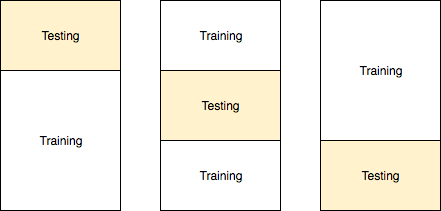
\includegraphics[width=1\linewidth]{adit_pics/cross_validation}
	\caption{K-Fold \textit{cross validation} dengan nilai k=3}
	\label{fig:cross_val}
\end{figure}

Pada K-Fold \textit{cross validation}, variabel K akan digantikan dengan nilai yang menunjukan pembagian dari \textit{training} dan \textit{testing} yang akan dilakukan. Pada contoh gambar dengan k=3, keseluruhan data akan dibagi menjadi 3 bagian, lalu 1 bagian tersebut akan digunakan untuk \textit{testing} dan sisanya digunakan sebagai \textit{training}. Hal ini dilakukan sebanyak K kali, yang mana pada contoh gambar dilakukan sebanyak 3 kali. Hasil perhitungan F-Score nantinya akan diambil rata-ratanya dari setiap iterasi \textit{cross validation}.
%!TEX root = skripsi.tex
%-----------------------------------------------------------------------------%
\chapter{\babTiga}
%-----------------------------------------------------------------------------%
Bab ini akan menjelaskan gambaran proses penelitian secara keseluruhan yang terdiri dari pembuatan \textit{sense tagged corpus} bahasa Inggris,  \textit{word alignment} korpus paralel, peningkatan kualitas dan evaluasi \textit{word alignment}, pemindahan \textit{sense} dari korpus bahasa Inggris, dan sistem WSD yang diimplementasikan. Diagram dari rancangan sistem yang akan dibuat pada penelitian ini dapat dilihat pada gambar berikut:

\begin{figure}
	\centering
	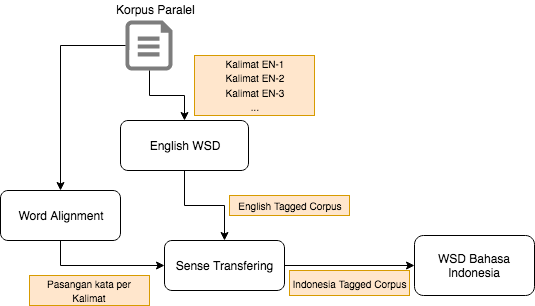
\includegraphics[width=1\linewidth]{adit_pics/WSD-full}
	\caption{Rancangan Sistem}
	\label{fig:Rancangan-Sistem}
\end{figure}
%-----------------------------------------------------------------------------%


\section{Korpus Identik}
Korpus utama yang digunakan sebagai sumber data penelitian ini adalah korpus identik. Korpus identik berisi pasangan kalimat-kalimat dalam bahasa Indonesia dan Inggris. Kalimat yang berpasangan di dalamnya sebagian besar mempunyai makna konten yang paralel walaupun terdapat juga yang \textit{comparable}. Korpus identik ini mempunyai 88.918 buah pasangan kalimat di dalamnya.


\section{Pembuatan \textit{Sense Tagged Corpus} Bahasa Inggris}
%-----------------------------------------------------------------------------%

Pembuatan \textit{sense tagged corpus} bahasa Inggris dilakukan dengan menggunakan \textit{tool} IMS untuk mendapatkan makna terbaik yang dapat ditag oleh \textit{tool} tersebut. Makna kata hasil dari proses ini akan dipindahkan ke kata yang bersesuaian pada kalimat yang sama pada bagian \textit{sense transfering}. \textit{File} yang diberikan sebagai masukan dari IMS adalah kalimat-kalimat pada bahasa Inggris yang berasal dari korpus identik.
%-----------------------------------------------------------------------------%
\section{\textit{Word alignment} pada Korpus Paralel}
%-----------------------------------------------------------------------------%
\textit{Word alignment} pada korpus berbahasa Inggris dan Indonesia menggunakan \textit{tools word alignment} bernama Giza++. \textit{Tool} ini merupakan salah satu \textit{word alignment tools} pada \textit{statistical machine translation} (SMT) yang dapat digunakan untuk memasangkan kata-kata pada dua buah korpus atau lebih. Terdapat beberapa \textit{word alignment tools} lain seperti Berkeley \textit{aligner}, anymalign, dan lain-lain. Penyelarasan kata ini digunakan untuk kebutuhan pemindahan \textit{sense} dari kata bahasa Inggris ke kata dalam bahasa Indonesia.

Proses \textit{alignment} yang dilakukan dengan Giza++ meliputi tahap-tahap berikut:
\begin{enumerate}
	\item Mempersiapkan kedua buah \textit{file} yaitu korpus bahasa asal (\textit{source}) dan korpus bahasa tujuan (\textit{target}). Kedua \textit{file} ini berpasangan dalam setiap barisnya. Baris pertama dalam \textit{file} pertama berpasangan dengan baris pertama pada \textit{file} kedua sampai akhir baris pada kedua \textit{file}.
	\item Menghasilkan \textit{file} perbendaharaan kata dari kedua bahasa dan \textit{list} indeks perbendaharaan kata pada tiap kalimat yang sudah diselaraskan
	\item Menghasilkan \textit{cooccurence file} dari kosa kata dan pasangan kalimat tersebut
	\item Proses \textit{alignment} yang menghasilkan beberapa macam \textit{output file} 
\end{enumerate}

Terdapat satu buah \textit{output file} Giza++ yang berisi pasangan-pasangan kalimat dengan kata-kata yang sudah diselaraskan dengan translasinya dalam bahasa tujuan. Hasil ini merupakan \textit{best viterbi alignment} menurut Giza++.

Pada skenario \textit{alignment} dengan bahasa Indonesia sebagai \textit{source} dan bahasa Inggris sebagai \textit{target}, satu kata dalam bahasa Indonesia akan dipasangkan dengan tepat satu kata dalam bahasa Inggris.

%-----------------------------------------------------------------------------%
\section{Evaluasi \textit{Word Alignment}} \label{sec:pembentukanTdanH}
%-----------------------------------------------------------------------------%
\textit{Word alignment} hasil dari \textit{tool} Giza++ dievaluasi dengan menggunakan \textit{anotator} hasil \textit{alignment} dari \textit{anotator} yang akan ditujukan sebagai \textit{gold standard}. Nilai-nilai yang akan dihitung meliputi \textit{precision} (P), \textit{recall} (R), dan F-\textit{score}. Metode evaluasi keseluruhan meliputi:

\begin{enumerate}
	\item Pemilihan \textit{random sampling} sebanyak dua ratus buah pasangan kalimat
	\item Masing-masing \textit{anotator} memasang-masangkan kata yang tepat pada masing-masing pasangan kalimat, dengan asumsi bahwa anotasi manusia sebagai \textit{gold standard}
	\item Hasil anotasi manusia dan keluaran dari \textit{tool} Giza dibandingkan untuk mendapatkan ketiga nilai P, R, F-Score, dan \textit{agreement} kedua anotator.
\end{enumerate}


%-------%
\section{Peningkatan Kualitas Hasil \textit{Alignment}}
%-----------------------------------------------------------------------------%
Proses peningkatan kualitas hasil alignment diperlukan untuk meminimalisir kesalahan pemasangan kata-kata pada proses sebelumnya. Permasalahan  yang terjadi adalah adanya pasangan-pasangan kata yang tidak benar seperti pada halnya kata "lapangan" misalnya yang  dipasangkan dengan kata dalam bahasa inggris \textit{field}, \textit{ground}, \textit{involved}, \textit{job}, \textit{program}, dan beberapa kata lainnya. Peningkatan kualitas \textit{alignment} ini dilakukan dengan dua buah pendekatan, yaitu dengan bantuan \textit{online dictionary} bahasa Indonesia-Inggris dan \textit{bi-directional alignment}. Pendekatan dengan bantuan kamus diterapkan dengan mencari kata terjemahan pada bahasa Inggris untuk menentukan apakah \textit{alignment} benar atau salah. Pada pendekatan kedua, dilakukan \textit{inverse} \textit{alignment} antara bahasa Indonesia ke Inggris. Jika pada proses awal \textit{alignment} dilakukan dengan menerapkan bahasa Indonesia sebagai \textit{source} dan Inggris sebagai \textit{target}, kali ini dilakukan proses yang berkebalikan. Pemanfaatkan hasil \textit{alignment} korpus bahasa Inggris ke Indonesia akan menghasilkan pasangan-pasangan kata dengan tingkat kesalahan \textit{alignment} lebih kecil dari \textit{alignment} satu arah saja. Metode yang akan dilakukan adalah dengan memeriksa setiap pasangan kata dari bahasa Indonesia yang mana merupakan kata dalam bahasa Inggris, apakah kata tersebut memiliki pasangan dalam \textit{inverse alignment} Giza.

%-----------------------------------------------------------------------------%
\section{\textit{Sense Transfering}} \label{sec:Sense Transfering}
%-----------------------------------------------------------------------------%
Pemindahan makna kata dilakukan dengan tiga buah \textit{sub-process} yang terdiri dari pemasangan antar kalimat, pemeriksaan kata, dan \textit{sense transfering}.
\begin{enumerate}
	\item Pemasangan antar kalimat yang bersesuaian dengan kata-kata yang berpasangan. Pada contoh kata "halaman" yang berpasangan dengan "courtyard", maka pasangan kalimat "Aku bermain di halaman" akan dipasangkan dengan kalimat "I play at the courtyard".
	\item Pemeriksaan untuk kata yang saling berpasangan dari hasil \textit{alignment} dan kamus hasil \textit{alignment enhancement}.
	\item \textit{Sense} dari kata yang menjadi \textit{target} tersebut kemudian diperiksa dengan \textit{sense} kata yang sama yang sudah pernah dipindahkan dari pasangan kalimat lain. 
	\item Jika \textit{sense} yang ingin dipindahkan "mirip" dan memiliki kedekatan makna dibatas \textit{threshold}, maka \textit{sense} yang akan dipindahkan hanya salah satu saja. Proses ini diperlukan untuk meminimalisir adanya satu kata bahasa Indonesia yang mempunyai lebih dari satu \textit{sense} yang mirip dari definisi makna tersebut.
	\item Bila "courtyard" memiliki \textit{sense} yang artinya adalah "halaman rumah", maka "halaman" pada kalimat "Aku bermain di halaman" memiliki \textit{sense} "halaman rumah".
\end{enumerate}

\section{Sistem WSD} \label{sec:Sistem WSD}
%-----------------------------------------------------------------------------%
Sistem WSD yang dibangun adalah dengan menggunakan pendekatan \textit{supervised learning}. Hasil dari pemindahan makna kata akan digunakan sebagai \textit{training} dan \textit{testing} data untuk menguji performa dari sistem yang dibangun. \textit{Classifier} yang digunakan dalam sistem \textit{WSD} ini adalah SVM. Pengujian dilakukan dengan menggunakan beberapa fitur seperti \textit{bag of words}, \textit{POS Tag}, dan \textit{word embedding}. Fitur \textit{bag of words} menggunakan \textit{window} sebanyak dua buah kata kanan dan kiri kata tujuan sebagai kata konteks. \textit{POS Tag} dan vektor \textit{word embedding} juga akan diimplementasikan pada penelitian ini. Performa dari sistem WSD akan dilihat berdasarkan perhitungan F1-score \textit{micro} dari hasil klasifikasi.
%!TEX root = skripsi.tex
%-----------------------------------------------------------------------------%
\chapter{\babEmpat} \label{implementasi}
%-----------------------------------------------------------------------------%
Bab ini akan menjelaskan perihal implementasi dari rancangan yang sudah dibuat pada bab sebelumnya.

\section{Pre-Processing}
Perlu dilakukan \textit{pre-processing} untuk memisahkan kalimat bahasa Inggris dan bahasa Indonesia dari korpus identik menjadi dua buah \textit{file} paralel untuk dapat diproses pada tahap-tahap berikutnya.

\begin{figure}
	\centering
	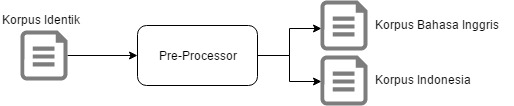
\includegraphics[width=1\linewidth]{adit_pics/pre-process-giza}
	\caption{Pre-Processing Giza}
	\label{fig:Pre-Processing-Giza}
\end{figure}


\section{Pembuatan \textit{Sense Tagged Corpus} Bahasa Inggris}
\textit{Sense Tagged Corpus} dibuat dengan menggunakan bantuan IMS untuk memberikan tag pada korpus bahasa Inggris. \textit{Pre-processing} dilakukan terlebih dahulu terhadap korpus bahasa Inggris seperti menghilangkan tanda baca dan mengubah semua token menjadi huruf kecil. Proses \textit{tagging} dilakukan dengan menjalankan perintah:

\begin{lstlisting}[language=bash, caption={IMS}, label={IMS}]
./testPlain.bash <model> <file_input> <file_output> <file_index_sense>
\end{lstlisting}

model yang digunakan IMS pada penelitian ini adalah model yang tersedia pada \textit{website software NUS} berdasarkan versi Wordnet 3.0. Model yang digunakan tersebut meliputi hasil \textit{training} kata-kata dalam bahasa Inggris yang sudah dilakukan di penelitian IMS. Proses yang dilakukan IMS dalam melakukan \textit{tagging sense} adalah dengan mengiterasikan melakukan \textit{sentence splitter}, \textit{tokenizing}, \textit{POS Tagging}, dan \textit{lemmatizing}. Setelah proses itu dilakukan, ekstraksi fitur dilakukan sebelum hasilnya masuk ke dalam \textit{classifier} berdasarkan model kata yang sudah ada. 


Hasil \textit{output} dari \textit{tool} tersebut adalah korpus dengan kata-kata sudah ditag dengan maknanya yang bersesuaian (dalam bentuk \textit{sense key}). \textit{Sense key} merupakan \textit{identifier} unik yang menyimpan arti dari suatu kata pada Wordnet Princeton. Untuk mempermudah pemakaian \textit{sense tagged corpus} ini pada proses selanjutnya, dilakukan \textit{post-processing} untuk mengubah hasil keluaran ke dalam format berikut:

\begin{lstlisting}
<sentence>kata-1||sensekey-1 kata-2||sensekey-2 ...</sentence>
<sentence>kata-n||sensekey-n kata-m||sensekey-m ...</sentence>
...
\end{lstlisting}

Contoh dari kalimat yang sudah diberikan \textit{tag} sampai keluar dari \textit{post-processing} adalah:

\begin{lstlisting}
<sentence>years||year%1:28:01:: animals||animal%1:03:00:: have||have%2:40:04:: caused||cause%2:36:00:: havoc||havoc%1:04:00::</sentence>
\end{lstlisting}

Pada contoh tersebut, kata years memiliki \textit{sense key} berupa "year\%1:28:01::", dimana berdasarkan Wordnet mempunyai arti sebagai '\textit{a period of time containing 365 (or 366) days}'. Tidak semua kata dalam korpus bahasa Inggris ditag oleh IMS, kata-kata sapaan seperti "I", "you", "a" , "the", dan beberapa kata lainnya tidak diberikan \textit{sense key}.  



\section{\textit{Word Alignment}}

\subsection{Pemrosesan \textit{Word Alignment}}
Proses \textit{word alignment} menggunakan dua buah \textit{file} yaitu korpus berbahasa Indonesia dan Inggris yang sudah dipisah dari \textit{pre-processing}. Perintah berikut digunakan untuk melakukan \textit{word alignment} dengan Giza pada penelitian ini:

\begin{lstlisting}[language=bash,caption={Word Alignment}, label={word-alignment}]
# Lakukan pada direktori Giza
./plain2snt.out [source_language] [target_language]

# proses diatas menghasilkan tiga buah file yaitu dua buah file vocabulary yang berisi indeks dengan kata (bahasa asal, dan bahasa tujuan), dan satu buah file snt yang berisi \textit{alignment} dari kalimat.

./snt2cooc.out [source_language_vcb_file] [target_language_vcb_file] [snt_file] > [coocurrence_file]

# proses snt2cooc akan menghasilkan \textit{cooccurence file}

./GIZA++ -S [source_language_vcb] -T [target_language_vcb] -C [snt_file] -CoocurrenceFile [cooc_file]
\end{lstlisting}

Giza mengeluarkan beberapa \textit{file} hasil dari proses tersebut. \textit{Output} yang akan digunakan diantaranya adalah \textit{file} bernama A3.final yang merupakan pasangan kalimat dengan kata-kata yang sudah dipasangkan sesuai dengan prediksi terbaik hasil pemrosesan Giza.

\subsection{Post-Processing}
Setelah mendapatkan \textit{file} A3 dari Giza, dilakukan \textit{post-processing} untuk menghasilkan file yang dengan mudah dapat diproses untuk melakukan \textit{sense transfering}.

Berikut ini merupakan salah satu contoh pasangan kalimat pada \textit{file} A3 keluaran Giza:

\begin{lstlisting}caption={A3-File}, label={a3-file}]
# Sentence pair (47183) source length 9 target length 9 alignment score : 6.85298e-13
Undang-Undang No 14 tahun 2008 tentang Kebebasan Memperoleh Informasi 
NULL ({ }) Law ({ 1 }) No ({ 2 }) 14 ({ 3 }) of ({ }) 2008 ({ 4 5 }) on ({ 6 }) Freedom ({ 7 8 }) of ({ }) Information ({ 9 })
\end{lstlisting}

Pembacaan pasangan kata berdasarkan hasil keluaran dilakukan dengan indeks nomor kata yang berada pada dalam kurung kata di bahasa Inggris. Karena pemisah token \textit{by default} adalah spasi, maka kata "Undang-Undang" adalah kata dengan indeks nomor 1, kata "No" adalah kata dengan indeks nomor 2, dan berlaku hal yang sama sampai kata "Informasi". Pada kata bahasa inggris, "Law" dipasangkan dengan indeks satu yang mana adalah "Undang-Undang", kata "No" dipasangkan dengan indeks dua yang mana adalah "No". 

Terdapat dua buah \textit{post-processing} yang dilakukan dengan tujuan masing-masing untuk:

\begin{enumerate}
	\item Penyimpan pasangan kata-kata yang bersesuaian untuk sistem WSD.
	\item Sebagai \textit{resource} untuk proses \textit{enhancement word alignment}.
\end{enumerate}


Untuk keperluan nomor satu, bentuk \textit{output} diproses menjadi bentuk lain dengan format:

\begin{lstlisting}
<pair>kata_en_1||kata_id_1 kata_id_2</pair?##<pair>kata_en_2||kata_id\_3</pair>...</pair>
\end{lstlisting}

Contoh dari hasil \textit{post-processing} pada pasangan kalimat sebelumnya adalah:

\begin{lstlisting}
<pair>law||undang-undang</pair>##<pair>no||no</pair>##<pair>14||14</pair>##<pair>2008||tahun 2008</pair>##<pair>on||tentang</pair>##<pair>freedom||kebebasan memperoleh</pair>##<pair>information||informasi</pair>
\end{lstlisting}

Hasil ini kemudian disimpan sebagai sebuah \textit{file} sendiri yang akan digunakan kembali pada sistem WSD nantinya. Sementara itu, keperluan nomor dua difokuskan untuk membuat \textit{dictionary} yang akan ditingkatkan kualitasnya pada tahap berikutnya. Untuk menghasilkan \textit{file} yang dibutuhkan pada nomor kedua, dilakukan pengumpulan pasangan kata bahasa Indonesia dengan bahasa Inggris. Bila misalkan pada kalimat ke-n terdapat kata "undang-undang" yang dipasangkan dengan "law", dan pasangan kata "undang-undang" dengan "regulation" pada kalimat lain (kalimat ke-m, dimana m != n). Berdasarkan kedua kalimat tersebut, maka kata "undang-undang" akan berpasangan dengan dua kata yaitu "law", dan "regulation".


\section{Evaluasi \textit{Word Alignment}}

\subsection{Pre-Processing}
Pertama, dilakukan pemilihan acak terhadap 200 pasang kalimat yang merupakan hasil keluaran Giza(\textit{file} A3). Setiap pasang tersebut meliputi dua buah isi yaitu kalimat bahasa Indonesia, dan kalimat bahasa Inggris dengan tanda \textit{alignment} Giza. Proses selanjutnya adalah menyiapkan 200 pasang kalimat tersebut untuk dievaluasi oleh anotator. Terdapat beberapa proses dalam mempersiapkan data untuk evaluasi oleh anotator.
\begin{enumerate}
	\item Pertama, pada setiap kata dalam bahasa Indonesia diberikan sebuah tanda indeks berupa angka untuk mempermudah proses evaluasi anotator nantinya. Pada proses tersebut, kalimat "Aku ingin makan" sebagai perumpamaan, diubah menjadi "Aku(1) ingin(2) makan(3)". Angka tersebut diperuntukan untuk mempercepat dan mempermudah kerja anotator nanti untuk melihat pasangan kata dari kalimat bahasa Inggris.
	\item Kedua, kosongkan nomor indeks hasil \textit{alignment} Giza pada kalimat bahasa Inggris. Perumpamaan pada kalimat "NULL (\{  \}) i (\{ 1 \}) want (\{ 2 \}) to (\{  \}) eat (\{ 3 \})" akan berubah menjadi  "NULL (\{  \}) i (\{  \}) want (\{   \}) to (\{  \}) eat (\{  \})" yang nantinya akan diisi secara manual oleh anotator.
\end{enumerate}

\subsection{Proses Anotasi Data}
Setelah 200 buah pasangan kalimat(data) tersebut selesai dipersiapkan, anotator akan melakukan anotasi data (\textit{alignment}) secara manual dengan panduan yang diberikan oleh \saya. Panduan tersebut meliputi keterangan dari \textit{task word alignment}, format data yang diberikan dan cara pembacaannya, dan yang paling utama adalah cara melakukan proses \textit{alignment}. Panduan anotasi yang diberikan dapat dilihat di lampiran pada laporan ini.

\subsection{Evaluasi}
Evaluasi perhitungan \textit{precision}, \textit{recall}, f-score, dan \textit{agreement} dilakukan secara otomatis dengan program yang dibuat dengan algoritma berikut.

\begin{lstlisting}[language=Python, caption={Word Alignment Evaluation}, label={word-alignment-evaluation}]

def evaluate_bracket(list_giza, list_anotator):
	# evaluate per character
	numbers_anotator = len(list_anotator)
	numbers_giza = len(list_giza)
	match = 0
	if numbers_giza < numbers_anotator:
		# iterate through the numbers giza
		for n in list_giza:
			if n in list_anotator:
				match += 1
	else:
		# iterate through the numbers anotator
		for n in list_anotator:
			if n in list_giza:
				match += 1
	return (numbers_anotator, numbers_giza, match)

# given sentence which already been alignned from the first anotator (an1), second anotator(an2), and giza(giza)
matches, total_giza, total_anotator, total_giza_1, total_anotator_1 = 0, 0, 0, 0, 0
precision, recall = [[],[]], [[],[]]

for each sentence in sentences:
	for each token in sentence:
		(numbers_anotator, numbers_giza, match) = evaluate_bracket(an1(token), giza(token))
		(numbers_anotator_1, numbers_giza_1, match_1) = evaluate_brakcet(an2(token), giza(token))
		agreement = count_agreement(an1(token), an2(token))
		matches += match
		matches_1 += match_1
		total_giza += numbers_giza
		total_giza_1 += numbers_giza_1
		total_anotator += numbers_anotator
		total_anotator_1 += numbers_anotator_1
	agreement.append(agreement)
	precision[0].append(matches/total_giza)
	recall[0].append(matches/total_anotator)
	precision[1].append(matches_1/total_giza_1)
	recall[1].append(matches_1/total_anotator_1)

precision = average(precision[0])
recall = average(recall[0])
precision_1 = average(precision[1])
recall_1 = average(recall[1])
agreement = average(agreement)	

\end{lstlisting}

Berdasarkan cara perhitungan evaluasi tersebut, terdapat dua buah \textit{precision} dan \textit{recall} yang mana masing-masing menunjukan indikator penilaian untuk anotator pertama dan kedua.

\section{Peningkatan Kualitas \textit{Alignment}}

Hasil dari \textit{alignment} kata yang dilakukan Giza masih menghasilkan pasangan-pasangan kata yang tidak tepat. Untuk mengurangi jumlah pasangan kata yang salah tersebut, dilakukan \textit{enhancement} terhadap hasil pasangan kata dari Giza. Terdapat dua macam peningkatan kualitas \textit{alignment} yang digunakan pada penelitian ini, yaitu \textit{crawling based} dan \textit{bi-directional based}.

\subsection{Pendekatan \textit{Crawling}}

Konsep \textit{crawling} pada penelitian ini mengacu pada kebutuhan untuk \textit{filtering} hasil pasangan kata yang salah berdasarkan kamus Indonesia-Inggris. Karena keterbatasan \textit{resource digital} kamus tersebut, maka dibutuhkan pendekatan \textit{crawling} dari \textit{online dictionary} untuk mendapatkan pasangan kata yang benar. Salah satu \textit{online dictionary} yang dapat diakses dan memiliki hasil terjemahan yang cukup baik adalah \textit{website} sederet.com. \textit{Crawling} dilakukan dengan memeriksa setiap pasangan bahasa Inggris dari kata Indonesia hasil Giza, apakah pasangan kata tersebut berada pada hasil penerjemahan yang sesuai. Ilustrasi dari proses ini dapat dimodelkan dalam contoh berikut:

\begin{enumerate}
	\item Kata "halaman" memiliki pasangan bahasa Inggris hasil Giza yaitu  "\textit{courtyard}", \textit{"yard"}, \textit{"page"}, dan "\textit{lawn}".
	\item Gunakan \textit{crawler} untuk menerima hasil terjemahan dari kata "halaman" dalam bahasa Inggris
	\item \textit{Crawler} mendapatkan hasil kata "\textit{page}", dan "\textit{courtyard}".
	\item Berdasarkan kedua hasil tersebut, maka pasangan kata "halaman" yang dianggap benar adalah irisan dari kedua \textit{set} tersebut yaitu "\textit{page}" dan "\textit{courtyard}"
\end{enumerate}

\subsection{Pendekatan \textit{Bi-directional}}

Metode lain yang digunakan untuk meningkatkan kualitas \textit{aligment} yaitu dengan memanfaatkan \textit{bi-directional alignment}. Proses yang dilakukan adalah melakukan validasi terhadap kata-kata yang berpasangan  dari kedua korpus. Bagan dari \textit{enhancement} pada \textit{bi-directional} ini dapat dilihat pada gambar \ref{fig:Bidirectional-Enhancement}.

\begin{figure}
	\centering
	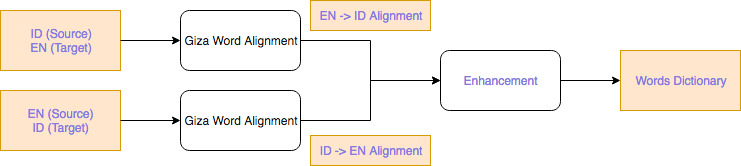
\includegraphics[width=1\linewidth]{adit_pics/bidirectional-enhancement}
	\caption{Bi-directional \textit{Enhancement}}
	\label{fig:Bidirectional-Enhancement}
\end{figure}

Pertama, setiap kata dalam bahasa Indonesia dikumpulkan terlebih dahulu dengan setiap pasangan kata bahasa Inggrisnya (satu kata bisa memiliki lebih dari satu pasangan). Proses selanjutnya adalah melakukan pengumpulan yang serupa terhadap kata dalam bahasa Inggris dengan pasangan kata dalam bahasa Indonesianya. Berbagai kata dalam bahasa Indonesia beserta pasangannya disimpan sebagai "kamus-1". Kata dalam bahasa Inggris, beserta pasangan kata Indonesianya disimpan sebagai "kamus-2". Proses validasi dilakukan dengan cara:

\begin{enumerate}
	\item Untuk setiap kata di bahasa Indonesia dalam "kamus-1" semisal kata "kali".
	\item Lakukan pengecekan terhadap setiap pasangan kata di bahasa Inggris pada "kamus-1" dari kata "kali", misalkan pasangan kata bahasa inggrisnya adalah "time", "river", dan "fire".
	\item Jika pada "kamus-2" kata "time" dipasangkan dengan "kali", dan "waktu" maka kata "time" merupakan pasangan yang dianggap benar (karena kata "time" berpasangan dengan "kali"). Pada kasus kata "fire", bila pasangan bahasa Indonesianya adalah "api" dan "tungku", maka kata "fire" dianggap bukan pasangan yang tepat dengan "kali" karena tidak terdapat pasangan "fire -> kali".
\end{enumerate} 

\begin{lstlisting}[language=Python, caption={Word Alignment Enhancement}, label={word-alignment-enhancement}]

dict_id = {}
dict_en = {}

# masukan setiap kosa kata bahasa Indonesia ke dalam dict_id sebagai key dan kumpulan pasangan kata bahasa inggrisnya sebagai value
# proses yang sama dilakukan untuk dict_en dengan kosa kata bahasa Inggris sebagai key dan kumpulan pasangan kata bahasa Indonesia sebagai value
# stop adalah list stopword yang didapat dari korpus nltk

# this section is for filtering which english word that has corresponding indo translation (bidirectional) from Giza output
for indo_word in dict_id.keys():
	for en_word in dict_id[indo_word].keys():
		if en_word != dict_en:
		# filtering so no same translation is entered, answer -> answer, jawaban -> jawaban
			if en_word in dict_en and indo_word in dict_en[en_word] and en_word not in stop:
				if indo_word not in final_dictionary:
					final_dictionary[indo_word] = { en_word: dict_en[word_en][word_id] }
				else:
					if en_word not in final_dictionary[indo_word]:
						final_dictionary[indo_word][en_word] = dict_en[word_en][word_id]
\end{lstlisting}

\section{\textit{Sense Transfering}}
Hasil dari proses peningkatan kualitas \textit{alignment} adalah sebuah "kamus" bahasa yang akan digunakan sebagai referensi untuk memindahkan makna kata dari bahasa Inggris ke kata yang benar pada bahasa Indonesia. Proses ini dilakukan dengan tahap-tahap sebagai berikut:

\begin{enumerate}
	\item Iterasi untuk setiap kata dalam bahasa Indonesia pada kamus
	\item Iterasi pada setiap pasangan kalimat
	\item Periksa apakah "\textit{pair}" kata bahasa Indonesia tersebut terdapat di dalam kamus
	\item Jika "pair" tersebut benar berada dalam kamus, maka pindahkan makna kata dari \textit{english word} yang bersesuaian.
\end{enumerate}

Ilustrasi dari proses tersebut pada kata "halaman" adalah sebagai berikut:

\begin{enumerate}
	\item Jika misalkan kata "halaman" pada kamus memiliki pasangan kata "page" dan "courtyard".
	\item Pada sebuah kalimat "... halaman kedua ..." dimana "\textit{pair}" pada kalimat tersebut diantaranya adalah
	\begin{lstlisting}
	..<pair>second||kedua</pair>##<pair>page||halaman</pair>..
	\end{lstlisting}
	\item Pasangan kata yang didapat dari "halaman" dari \textit{pair} tersebut adalah "page". Berdasarkan hasil tersebut kata "page" kemudian diperiksa kata dari \textit{pair} tersebut pada kamus.
	\item Karena kata "page" dari \textit{pair} terdapat pada kamus untuk kata "halaman", maka pindahkan makna "page" dari \textit{sense tagged corpus} kalimat tersebut ke kata "halaman" pada kalimat Indonesia dengan indeks yang sama.
\end{enumerate}

%-----------------------------------------------------------------------------%
\section{Sistem WSD}
Sistem WSD dibangun dengan menggunakan \textit{supervised learning}. \textit{Machine learning tool} yang digunakan untuk membangun sistem ini adalah Scikit \citep{scikit-learn}. Pada sistem ini terdapat tiga buah bagian utama yaitu pemilihan fitur serta \textit{classifier}, ekstraksi fitur, dan evaluasi hasil \textit{classifier}.

\subsection{Pemilihan Fitur dan \textit{Classifier}}
Terdapat tiga buah fitur pada penelitian ini yang terdiri dari:

\begin{enumerate}
	\item Fitur \textit{bag of words}
	\item Fitur \textit{POS tagging}
	\item Vektor dari hasil \textit{word embedding}
\end{enumerate}

\textit{Classifier} yang digunakan pada penelitian ini adalah SVM dengan \textit{library} Python yaitu Scikit dengan parameter \textit{default} berupa kernel linear dan C=1.

\subsection{Ekstraksi Fitur}
Fitur bag of words menggunakan pendekatan kemunculan kata-kata pada konteks kalimat sebagai fitur. Kata yang diambil untuk dijadikan fitur adalah dua buah kata di kiri dan di kanan dari \textit{target word}. Pada penelitian ini, kata-kata yang merupakan bagian dari \textit{stopwords} dalam bahasa Indonesia tidak dimasukan sebagai fitur. Contoh dari fitur ini dapat dilihat pada kalimat dengan kata tujuan "bisa" berikut:
\\
- Ani digigit ular dengan bisa yang berbahaya
\\
Pada contoh kalimat tersebut, \textit{bag of words} yang diambil adalah ["digigit", "ular", "berbahaya", NULL]

Setiap fitur \textit{bag of words} dari setiap kalimat tersebut dikumpulkan untuk menjadi satu fitur besar yang mendeteksi kemunculan kata-kata tersebut pada setiap kalimat.

Proses yang dilakukan dalam pengambilan kata konteks untuk fitur \textit{bag of words} dilakukan dengan tahap-tahap berikut.

\begin{lstlisting}[language=python,caption={Fitur Bag of Words}, label={fitur-bag-of-words}]

bag_of_words []

for each sentence
	split sentence by whitespace into words
	for each word
		if word == target word
			for x in [-2,-1,1,2]
				if word(x) exist and word(x) not in bag_of_words
					add word(x) into bag_of_words
					
return bag_of_words

\end{lstlisting}

Fitur POS Tagging menggunakan \textit{tool} dari Stanford bernama "A Part-Of-Speech Tagger" yang dilatih dengan menggunakan model untuk bahasa Indonesia. Proses \textit{tagging} ini dilakukan sebelum memasuki sistem WSD terhadap keseluruhan kalimat dalam korpus identik yang berisi bahasa Indonesia saja. Terdapat \textit{pre-processing} awal pada korpus bahasa Indonesia tersebut untuk menghilangkan beberapa tanda baca seperti titik, koma, tanda tanya, tanda seru, dan beberapa tanda baca lainnya. Setelah proses tersebut, diberikan tanda baca berupa titik pada akhir kalimat sebagai indikator akhir sebagai kebutuhan dari kompabilitas \textit{tool} (tidak semua kalimat pada korpus memiliki tanda baca akhir kalimat). Perintah yang dilakukan untuk melakukan \textit{POS Tagging} tersebut adalah:

\begin{lstlisting}[language=bash,caption={Stanford POS Tagger}, label={stanford-pos-tagger}]

java -mx300m -cp 'stanford-postagger.jar:lib/*' edu.stanford.nlp.tagger.maxent.MaxentTagger -model <model_bahasa_indonesia> -textFile <korpus_bahasa_indonesia>

\end{lstlisting}

Hasil dari proses tersebut merupakan korpus dengan setiap kata yang sudah memiliki POS Tag dengan format:

\begin{lstlisting}
<kata_1>_<postag_1> <kata_2>_<postag_2> ... <kata_n>_<postag_n>
<kata_x> <postag_x> <kata_y>_<postag_y> ... <kata_z>_<postag_z>
...
\end{lstlisting}

Kelas kata yang diambil adalah POS Tag dari \textit{target word} kata sebelum, dan kata sesudahnya. Kelas kata dari \textit{target word} diperhitungkan karena pada beberapa kasus kata polisemi dapat dibedakan maknanya berdasarkan POS Tag yang dimilikinya. POS Tag yang digunakan mengacu pada kelas-kelas yang ada pada POS Tag Penn Treebank seperti NN(Noun), NNP(Proper Noun), VB(verb), CC(Coordinating conjunction), dan lain-lain. Pembentukan kelas POS Tag untuk menjadi fitur dilakukan dengan proses yang serupa pada fitur \textit{bag of words} dimana kombinasi kombinasi dari POS Tag yang mungkin direpresentasikan dalam \textit{one hot representation}. Hal ini dapat diilustrasikan dengan proses berikut:

\begin{enumerate}
	\item Simpan POS Tag dari indeks kata masing-masing (\textit{target word}-1, \textit{target word}, \textit{target word}+1)
	\item Untuk masing-masing indeks baik itu -1,0,dan 1
	\item Kumpulkan POS Tag yang \textit{distinct}, populasikan dalam \textit{array}
	\item \textit{Array} ini nantinya akan merepresentasikan keberadaan POS Tag tertentu pada kata dengan indeks terkait tersebut
\end{enumerate}

Fitur ketiga yang dicoba adalah \textit{word embedding}. Model dari \textit{word embedding} yang digunakan sudah dilatih dengan menggunakan korpus Wikipedia bahasa Indonesia. Vektor \textit{word embedding} yang dijadikan fitur adalah vektor dari semua kata pada kalimat tersebut. Semua vektor nilai dari kata-kata tersebut kemudian dikonkatenasi menjadi satu buah vektor besar. Untuk menjamin panjang vektor yang sama untuk setiap kalimat, panjang vektor disesuaikan dengan kalimat terpanjang dari semua kalimat yang mengandung \textit{target word} tersebut. Proses tersebut dapat diilustrasikan pada gambar berikut:

\begin{figure}
	\centering
	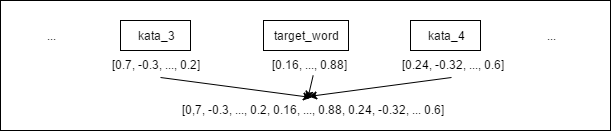
\includegraphics[width=1\linewidth]{adit_pics/we-vector}
	\caption{Ilustrasi Fitur Word Embedding}
	\label{fig:Ilustrasi-Fitur-Word-Embedding}
\end{figure}


\subsection{Evaluasi Sistem}
\textit{Target word} untuk evaluasi dipilih secara manual yang memenuhi kriteria bahwa kata tersebut memiliki kata \textit{translation} lebih dari satu dengan makna yang berbeda.Evaluasi dilakukan dengan \textit{cross validation} menggunakan perhitungan F1-score dari hasil klasifikasi yang dilakukan \textit{classifier} terhadap \textit{target word}. \textit{Cross validation} dilakukan dengan iterasi sebanyak tiga kali dengan perbandingan antara \textit{training} dan \textit{test set} sebesar 0,7:0,3.

Sebuah algoritma sederhana digunakan sebagai \textit{baseline} untuk pembanding dari sistem WSD yang dibangun. Baseline menggunakan pendekatan \textit{most frequent sense} sebagai cara untuk menentukan makna terbaik dari suatu kata. Bila diberikan \textit{training data} untuk kata "bisa" dengan makna "dapat melakukan" sebanyak 4 buah dan makna "racun ular" sebanyak 6 buah, maka algoritma baseline ini akan mengklasifikasikan semua kata "bisa" menjadi "racun ular".


%!TEX root = skripsi.tex
%-----------------------------------------------------------------------------%
\chapter{\babLima}
%-----------------------------------------------------------------------------%
Bab ini menjelaskan mengenai hasil yang didapatkan dari eksperimen, serta evaluasi dan analisis terkait hasil tersebut.

%-----------------------------------------------------------------------------%
\section{\textit{Sense Tagged Corpus} Bahasa Inggris}
Tabel \ref{table:sense-tagged-corpus} menunjukan jumlah token (kata) pada korpus bahasa Inggris dan yang diberikan \textit{tag sense} oleh IMS

\begin{table}
	\centering
	\caption{Jumlah \textit{instance} korpus bahasa Inggris}
	\label{table:sense-tagged-corpus}
	\begin{tabular}{|p{0.7cm}|p{4cm}|p{4cm}|}
		\hline
		No & Tipe & Jumlah
		\\ \hline
		1    & 
		Token (kata)   & 
		1.801.484
		\\ \hline
		2    & 
		Kata yang diberikan \textit{tag} oleh IMS     & 
		1.024.797 
		\\ \hline
	\end{tabular}
\end{table}

Berdasarkan proses pembuatan dan hasil dari \textit{sense tagged corpus} tersebut, dapat dilihat bahwa tidak semua kata diberikan \textit{sense} oleh IMS. Kata-kata sapaan seperti "I", "you", dan kata \textit{articles} yaitu "a", "the", "an". Tingkat kebenaran dari \textit{sense tag} yang diberikan bergantung dari model yang digunakan pada penelitian. Terdapat banyak kasus-kasus dimana pemberian \textit{sense} yang dilakukan adalah benar seperti misalnya pada kata "\textit{visitor}" yang diberikan \textit{tag} dengan \textit{sense key} 1:18:00::, yang mana berdasarkan wordnet Princeton "visitor\%1:18:00::" memiliki arti sebagai "\textit{someone who visits}". Contoh lain dari kata yang diberikan \textit{tag} dengan benar adalah "\textit{company}" pada konteks potongan kalimat "\textit{Plantation company PT ...}". Kata "\textit{company}" tersebut diberikan tag "company\%1:14:01::" yang berdasarkan wordnet Princeton memiliki makna "\textit{an institution created to conduct business}". Namun demikian, terjadinya kesalahan pemberian \textit{tag} pada kata terjadi pada kasus-kasus seperti: 

\begin{enumerate}
	\item Sebuah entitas diberikan \textit{tag} dimana entitas tersebut dianggap kata biasa. Contohnya adalah kata "Scotland Yard" dimana "Yard" pada kata tersebut diberikan \textit{tag} yang diartikan sebagai "\textit{a unit of length equal to 3 feet}". Hal ini menunjukan bahwa \textit{tool} belum dapat membedakan antara entitas yang memang tidak perlu diberikan \textit{tag} dan kata biasa (walaupun kata tersebut sudah memiliki huruf kapital).
	
	
	\item Kesalahan \textit{tag} dikarenakan \textit{training data} yang digunakan oleh model. Pada potongan kalimat "\textit{... FASB rule will cover such financial instruments as interest rate swaps financial ...}, kata "\textit{interest}" diberikan tag dengan makan "a sense of concern with and curiosity about someone or something". Berdasarkan konteks kalimat tersebut, dapat diketahui bahwa makna yang seharusnya didapat untuk kata "\textit{interest}" di atas ialah "bunga bank". Percobaan untuk \textit{tagging} sense dari kalimat "bank interest is high" juga menghasilkan \textit{sense key} yang sama untuk kata \textit{interest} (mendapatkan \textit{sense key "keingintahuan"}) walaupun pada kalimat tersebut makna yang seharusnya didapat adalah "bunga bank".
		
	\item Pemberian \textit{tag} pada \textit{multi word} token seperti "\textit{make up}" masih diberikan pada setiap kata ("\textit{make}" dan "\textit{up}" memiliki \textit{sense key} masing-masing). Hal ini terjadi karena IMS mengolah kata demi kata dengan proses tokenisasi \textit{by default} menggunakan spasi. Setelah dilakukan pemeriksaan pada kata-kata yang terdapat pada model, kata \textit{make up} ternyata disimpan sebagai "make\_up". Berdasarkan pemeriksaan tersebut, dapat disimpulkan bahwa IMS dapat melakukan \textit{tagging} yang benar dari kata "make up" jika dijadikan satu buah token berupa "make\_up". hasil \textit{tagging} yang benar untuk kasus seperti kata-kata tersebut memerlukan \textit{pre-processing} untuk mengganti \textit{separator} kata multiword yang umumnya menggunakan spasi dengan "\_" agar IMS dapat memberikan \textit{tag multi word} tersebut dengan benar. Selain \textit{pre-processing},  IMS juga dapat melakukan \textit{tagging} dengan input dalam format XML. Bentuk kata-kata dan kalimat dalam format XML tersebut biasanya memiliki \textit{multi word} yang sudah dijadikan satu token sehingga mempermudah penyelesaian masalah tersebut.
\end{enumerate}
%-----------------------------------------------------------------------------%

%-----------------------------------------------------------------------------%
\section{\textit{Word Alignment}}

Proses alignment dilakukan terhadap semua pasangan kalimat pada korpus identik (total sebanyak 88.919 buah). Hasil dari proses \textit{word alignment} yang dilakukan Giza dibandingkan dengan hasil \textit{alignment} yang dibuat oleh dua orang anotator. Jumlah yang akan dibandingkan adalah 200 buah pasangan data yang didapat dengan \textit{random sampling}. Indikator performa dari perbandingan tersebut adalah nilai dari \textit{precision}, \textit{recall}, dan F-score sesuai dengan penyesuaian cara perhitungan dari penelitian \citep{mihalcea2003evaluation}. Hasil evaluasi yang didapatkan dapat dilihat pada tabel \ref{table:word-alignment-evaluation}

\begin{table}
	\centering
	\caption{Evaluasi Word Alignment}
	\label{table:word-alignment-evaluation}
	\begin{tabular}{|p{2cm}|p{2cm}|p{2cm}|p{2cm}|}
		\hline
		\textbf{Anotator} & \textbf{Precision} & \textbf{Recall} & \textbf{F-Score}
		\\ \hline
		1 & 0.775 & 0.747 & 0.761
		\\ \hline
		2 & 0.768 & 0.75 & 0.759
		\\ \hline
	\end{tabular} 
\end{table}

\textit{Agreement} antara kedua anotator pada \textit{random sampling alignment} adalah 0.924.

Evaluasi hasil anotasi tersebut juga dilihat dari sisi perbandingan jumlah \textit{alignment} yang \textit{exact match} dengan total kata. Suatu \textit{alignment} dikatakan sebagai \textit{exact match} jika pasangan kata yang diberikan oleh kedua anotator sama persis. Contoh yang tidak \textit{exact match} adalah jika misalkan kata "keluar" dipasangkan dengan "\textit{get out}" pada anotator 1, namun dipasangkan dengan "\textit{out}" pada anotator 2. \textit{Alignment} dikatakan \textit{exact match} pada kasus sebelumnya jika anotator 2 juga memasangkan kata "keluar" dengan "\textit{get out}". Jumlah dan perbandingan \textit{exact match} antara kedua anotator dengan total pasangan kata dapat dilihat pada tabel \ref{table:exact-match-anotator}.

\begin{table}
	\centering
	\caption{Perbandingan \textit{exact match alignment} anotator}
	\label{table:exact-match-anotator}
	\begin{tabular}{|p{3cm}|p{3cm}|p{3cm}|}
		\hline
		\textbf{\textit{Exact match} (e)} & \textbf{Total \textit{alignment} (t)} & \textbf{Rasio (e/t)}
		\\ \hline
		4.315 & 5198 & 0.83 \\ \hline
	\end{tabular} 
\end{table}
 
Perbandingan antara jumlah \textit{alignment} yang \textit{exact match} antara kedua anotator dengan pasangan kata pada 200 \textit{sample} yang diberikan adalah 0.83. Hal ini berarti 83\% dari \textit{alignment} yang dilakukan kedua anotator memiliki kesamaan pasangan kata yang identik.

Berdasarkan hasil beberapa analisis \textit{word alignment} tersebut, dapat dilihat bahwa Giza++ secara umum dapat menghasilkan \textit{alignment} pada korpus identik dengan nilai F-Score sekitar 75\%. Namun demikian, kesalahan yang terjadi pada \textit{alignment} Giza ada di kasus-kasus seperti:

\begin{enumerate}
	\item Pemasangan frasa kompleks dengan kata lain. Seperti misalnya frasa "\textit{a very awesome and huge building}" dengan "gedung raksasa", ataupun gaya bahasa lainnya yang menjadikan frasa tersebut kompleks dan panjang.
	\item Pasangan kalimat yang tidak sepenuhnya paralel (\textit{comparable}), seperti misalnya "I'm glad that you're here" dengan "Aku senang kau ada". Variasi dari bentuk kalimat \textit{comparable} terkadang mempersulit model dari Giza++ untuk menentukan pasangan kata yang benar.
\end{enumerate}

Walaupun akurasi yang didapatkan sekitar 70\%, tidak jarang ditemukan pasangan kata-kata yang tidak sesuai dan dapat menjadi masalah pada saat \textit{sense transfering} sehingga dilakukan proses \textit{word alignment enhancement}.

Hasil \textit{enhancement} dengan pendekatan \textit{bi-directional} masih menghasilkan kata-kata yang memiliki pasangan tidak sesuai seperti misalnya kata "pembuat" dengan "\textit{jewelry}", kata "pendidikan" dengan "\textit{tended}", kata "harapkan" dengan "\textit{anticipate}", dan lain-lain. Skenario pada \textit{enhancement} menggunakan \textit{crawling} kamus Indonesia-Inggris tidak menghasilkan pasangan yang salah seperti pada contoh yang diberikan di atas. Evaluasi terhadap hasil \textit{enhancement} ini dilakukan dengan mengambil 10 buah \textit{sample} secara \textit{random} dari pasangan kata yang ada. Hasil \textit{sampling} tersebut dapat dilihat pada \ref{table:random-sampling-enhancement}.

\begin{table}
	\centering
	\caption{Pasangan kata hasil \textit{random sampling} dengan pendekatan \textit{bi-directional} dan \textit{crawling}}
	\label{table:random-sampling-enhancement}
	\begin{tabular}{|p{4cm}|p{4cm}|p{4cm}|}
		\hline
		\textbf{Kata} & \textbf{\textit{Bi-directional}} & \textbf{\textit{Crawling}}
		\\ \hline
		memodernkan & \textit{modernize} & \textit{modernize} \\ \hline
		kembar & \textit{twin}, \textit{twins} & \textit{twin}, \textit{twins} \\ \hline
		ingat & \textit{remember}, \textit{remembered}, \textit{recall}, \textit{note}, \textit{recalls}, \textit{strike} & \textit{remembered}, \textit{recall}, \textit{remember} \\ \hline
		peroksida & peroxide & peroxide \\ \hline
		imbang & \textit{draw}, \textit{drawing} & \textit{draw}, \textit{drawing} \\ \hline
		tegang & \textit{tense}, \textit{edge} & \textit{tense} \\ \hline
		berobat & \textit{medical}, \textit{purpose}, \textit{treatment} & \textit{treatment} \\ \hline
		membantu & \textit{bolster}, \textit{supporting}, \textit{beneficial}, \textit{helping}, \textit{help}, \textit{support}, \textit{assisted}, \textit{assist}, \textit{appearance}, \textit{assisting}, \textit{helped}, \textit{assists}, \textit{helps}, \textit{aiding}, \textit{aid}, \textit{facilitates}, \textit{supports}, \textit{assistance} & \textit{helped}, \textit{assisting}, \textit{facilitating}, \textit{help}, \textit{assisted}, \textit{assist}, \textit{helpful}, \textit{helping}, \textit{helps}, \textit{aid}, \textit{facilitates}, \textit{supports}, \textit{avail} \\ \hline
		disusun & \textit{composed}, \textit{arranged}, \textit{developed}, \textit{structured}, \textit{organized}, \textit{prepared}, \textit{compiled} & \textit{composed}, \textit{arranged}, \textit{developed}, \textit{structured}, \textit{prepared}, \textit{compiled} \\ \hline
		diusulkan & \textit{suggested}, \textit{suggests}, \textit{recommended}, \textit{proposed}, \textit{proposes} & \textit{suggested}, \textit{proposed} \\ \hline
	\end{tabular}
\end{table}

Pasangan kata pada tabel di atas kemudian dihitung berapa jumlah pasangan yang benar untuk masing-masing pendekatan (\textit{bi-directional} dan \textit{crawling}). Pasangan kata dianggap benar jika hasil translasi kata tersebut dapat digunakan untuk konteks kalimat tertentu. Hasil evaluasi dengan mengukur precision dari hasil tersebut dapat dilihat pada tabel \ref{table:enhancement-precision}.


\begin{table}
	\centering
	\caption{Precision dari hasil \textit{random sampling alignment enhancement}}
	\label{table:enhancement-precision}
	\begin{tabular}{|p{2.5cm}|p{3cm}|p{3cm}|}
		\hline
		\textbf{Kata} & \textbf{\textit{Bi-directional}} & \textbf{\textit{Crawling}}
		\\ \hline
		memodernkan & 1.0 & 1.0 \\ \hline
		kembar & 1.0 & 1.0 \\ \hline
		ingat & 0.67 & 1.0 \\ \hline
		peroksida & 1.0 & 1.0 \\ \hline
		imbang & 0.5 & 0.5 \\ \hline
		tegang & 1.0 & 1.0 \\ \hline
		berobat & 0.33 & 1.0 \\ \hline
		membantu & 0.73 & 0.84 \\ \hline
		disusun & 0.71 & 0.66 \\ \hline
		diusulkan & 0.6 & 1.0 \\ \hline	
		\hline
		\textbf{Rata-rata} & 0.78 & 0.90 \\ \hline
	\end{tabular}
\end{table}

Berdasarkan evaluasi pada tabel di atas, didapatkan bahwa pendekatan \textit{crawling} pada \textit{random sampling} tersebut memiliki tingkat precision yang lebih tinggi dari \textit{bi-directional} yaitu sebesar 90\%. Kamus hasil dari \textit{crawling} inilah yang akan digunakan untuk proses \textit{sense transfering}.

%-----------------------------------------------------------------------------%
\section{\textit{Sense Transfering}}

Proses \textit{transfer} makna kata dari bahasa Inggris ke bahasa Indonesia yang dilakukan sangat bergantung dari hasil \textit{alignment} kata pada proses sebelumnya. Untuk sebagian besar kata yang memiliki pasangan kata yang benar, proses \textit{transfer} dapat menghasilkan makna yang benar juga. Hal tersebut didukung jika \textit{sense tagged word} pada korpus bahasa Inggris juga benar). Terdapat beberapa kata yang dipilih sebagai \textit{sampling} untuk mengevaluasi hasil \textit{sense transfering}. Kelompok ini dibagi menjadi:

\begin{enumerate}
	\item Jumlah Kelas
	\begin{enumerate}
		\item 3-5 kelas kata
		\item lebih dari 5 kelas kata
	\end{enumerate}
	\item sebaran jumlah \textit{instance} dalam kelasnya
	\begin{enumerate}
		\item \textit{balance}
		\item \textit{imbalance}
	\end{enumerate}
	\item Bentuk morfologi dari kata tersebut
	\begin{enumerate}
		\item Lemma (kata dasar)
		\item Berimbuhan baik itu infleksional ataupun \textit{derivative}
	\end{enumerate}
\end{enumerate}

Pada laporan ini, hasil dari \textit{sense transfering} yang dianalisis adalah proses yang menggunakan kamus \textit{crawling}. Pada jumlah kelas sebanyak 3-5 kelas kata (\textit{sense key}), \textit{target word} yang diambil adalah "memecahkan". Kata tersebut memiliki 4 buah kelas total dengan \textit{sense key} yang didapat yaitu 'solve\%2:31:00::','resolve\%2:31:01::', 'break\%2:30:03::', dan 'split\%2:38:00::'. Kata "menolak" mewakili kelas kata sebanyak 9 buah yang diantaranya mengandung kelas 'reject\%2:40:00::', 'decline\%2:32:00::', rebuff\%2:32:00::, dan enam buah kelas lainnya. Makna kata 'decline\%2:32:00::' sendiri sebenarnya merupakan "gabungan" dengan 'refuse\%2:32:00' yang memiliki kemiripan dengan nilai \textit{path similarity} melewati batas \textit{threshold}, sehingga makna kata dianggap sama dan diberikan \textit{tag} sebagai 'decline' (dipilih satu \textit{tag} saja). Tabel \ref{table:number-classes-sense-transfering-evaluation} menunjukan contoh beberapa kata tersebut dalam beberapa konteks kalimat yang bersesuaian.

\begin{table}
	\centering
	\caption{Evaluasi \textit{Sense Transfering} Berdasarkan Jumlah Kelas}
	\label{table:number-classes-sense-transfering-evaluation}
	\begin{tabular}{|p{4cm}|p{4cm}|p{4cm}|}
		\hline
		\textbf{\textit{Sense Key}} & \textbf{Makna} & \textbf{Kalimat}
		\\ \hline
		solve\%2:31:00::  & 
		\textit{find the solution to (a problem or question) or understand the meaning of}   & 
		salah satu cara untuk \textbf{memecahkan} persoalan yang pelik...
		\\ \hline
		resolve\%2:31:01:: & 
		\textit{bring to an end / settle conclusively}   & 
		evolusionis masih belum bisa \textbf{memecahkan} permasalahan darwin...
		\\ \hline
		break\%2:30:03:: & 
		\textit{terminate}   & 
		...base mereka \textbf{memecahkan} rekor untuk...
		\\ \hline
		split\%2:38:00:: &
		\textit{go one's own way; move apart;} &
		senat mereka \textbf{memecahkan} perbedaan antara skenario 1 dan 3 dengan
		\\ \hline
		decline\%2:32:00:: &
		\textit{show unwillingness towards} &
		wells rich \textbf{menolak} untuk berkomentar...
		\\ \hline
		rebuff\%2:32:00:: &
		\textit{reject outright and bluntly} &
		georgia gulf \textbf{menolak} penawaran tersebut ...
		\\ \hline
		reject\%2:40:00:: &
		\textit{refuse to accept} &
		..dua pekan lalu \textbf{menolak} tawaran pemerintah...
		\\ \hline
	\end{tabular}
\end{table}

Makna kata \textit{split} yang diberikan hanya berjumlah satu buah dari keseluruhan korpus, hal ini disebabkan karena kata bahasa Inggris yang digunakan pada kalimat bahasa Inggrisnya menggunakan kata \textit{split}. Berdasarkan \textit{sampling} yang dilakukan, jumlah kelas kata yang ada bergantung pada sebanyak apa sebuah kata di bahasa Indonesia dipasangkan dengan kata bahasa Inggris yang berbeda dan memiliki makna pada \textit{sense tagged english corpus}. Jumlah kelas ini dapat bergantung pada seberapa akurasi \textit{alignment} kata yang dilakukan pada proses sebelumnya.

Pada sebaran jumlah \textit{instance} di dalam kelas-kelasnya, kata "kehadiran" memiliki jumlah kelas \textit{attendance} (19 buah), \textit{presence} (64 buah), dan \textit{existence
} 1 buah. Perbandingan kedua kelas dengan \textit{instance} terbanyak tersebut adalah 19:64 yaitu 0.29. Kedua \textit{sense} tersebut memiliki makna yang kurang lebih menyatakan sebuah \textit{state} dimana seseorang datang/hadir. Sementara itu, kelas kata "rumahnya" memiliki jumlah \textit{instance} sebanyak 32 buah pada kelas "house", dan 19 buah pada kelas "home". Perbandingan kedua kelas pada kata "rumahnya" tersebut adalah 0.59, yang mana rasio tersebut yang lebih besar dari rasio kelas kata "kehadiran" (0.29). Tabel \ref{table:class-instance-sense-transfering-evaluation} menunjukan makna kata yang dipindahkan berdasarkan \textit{sampling} berdasarkan sebaran \textit{instance} dalam kelas.

\begin{table}
	\centering
	\caption{Evaluasi \textit{Sense Transfering} Berdasarkan Sebaran Kelas}
	\label{table:class-instance-sense-transfering-evaluation}
	\begin{tabular}{|p{4cm}|p{2.85cm}|p{2.85cm}|p{1.2cm}|}
		\hline
		\textbf{Kata (\textit{sense key})} & \textbf{Makna} & \textbf{Kalimat} & \textbf{Jumlah}
		\\ \hline
		Kehadiran (attendance\%1:04:00::)  & 
		\textit{the act of being present (at a meeting or event etc.)}   & 
		...tingkat \textbf{kehadiran} guru di sekolah... &
		19
		\\ \hline
		Kehadiran (presence\%1:09:00::) & 
		\textit{the impression that something is present}   & 
		...berkurangnya \textbf{kehadiran} pria dewasa...
		&
		64
		\\ \hline
		rumahnya (house\%1:14:02::) & 
		\textit{an official assembly having legislative powers} & 
		...kebakaran yang melanda \textbf{rumahnya}...
		& 32
		\\ \hline
		rumahnya (home\%1:06:00::) &
		\textit{Housing that someone is living in} &
		...ia pulang ke \textbf{rumahnya} pada sabtu...
		& 19
		\\ \hline
	\end{tabular}
\end{table}

Kedua makna pada kata "kehadiran" memiliki makna yang relatif dekat dan sesuai dalam konteks kalimat kata tersebut muncul. Namun demikian, \textit{sense key} pada kata rumah yaitu "house\%1:14:02::" memiliki makna yang salah, dimana sense key yang lebih tepat semestinya adalah house\%1:06:01:: dengan makna "\textit{a building in which something is sheltered or located}". Kesalahan makna kata yang dipindahkan tersebut disebabkan karena kata \textit{house} pada korpus inggris diberikan tag 'house\%1:14:02::'. Kesalahan ini seperti yang sudah dijelaskan pada analisis \textit{tagging} IMS pada sub-bab Pembuatan \textit{Sense Tagged Corpus} Bahasa Inggris.


Kelompok \textit{sampling} lain adalah makna yang akan dilihat pada kata dengan bentuk morfologi yang berbeda. Kata "makan", "makanan", dan "memakan" merupakan kata yang mewakili kasus bentuk morfologi dalam bentuk lemma maupun berimbuhan. Pada kata "makan", \textit{sense key} yang diterima dari hasil \textit{transfer} adalah eat\%2:34:00:: yang memiliki makna "\textit{take in solid food}". Kata "makanan" pada kalimat-kalimat yang ada diberikan \textit{sense key} food\%1:03:00:: yang diartikan sebagai "\textit{any substance that can be metabolized by an animal to give energy and build tissue}". Kata "memakan" sendiri memiliki beberapa \textit{sense key} seperti consume\%2:34:02::, eat\%2:34:00::, dan feed\%1:13:00::. Dari \textit{sense key} yang didapat tersebut, consume\%2:34:02::("spend extravagantly") bukan merupakan \textit{sense} yang tepat (seharusnya memiliki makna mengonsumsi makanan), dan feed\%1:13:00:: ("\textit{food for domestic livestock}") yang semestinya adalah "memberikan makanan".

Terdapat beberapa kata-kata yang dipilih secara manual untuk dihitung akurasi dari kesesuaian \textit{tag} makna yang didapat. Kriteria pemilihan kata-kata sebagai \textit{sample} ini yaitu memiliki pasangan kata  dalam Bahasa Inggris dan makna kata lebih dari satu. Evaluasi ini akan menghitung seberapa banyak kelas-kelas makna kata yang benar dari hasil \textit{transfering} pada kata-kata pilihan tersebut. Hasil akurasi dari jumlah makna kata yang tepat dapat dilihat pada tabel \ref{table:akuras-kelas-makna-kata}.

\begin{longtable}{|p{1.8cm}|p{1.2cm}|p{5cm}|p{1.2cm}|p{1.5cm}|} 
	\hline
	\textbf{Kata} & \textbf{Jumlah \textit{sense key}} & \textbf{\textit{sense key}}  & \textbf{Jumlah \textit{sense key} yang benar} & \textbf{Akurasi} \\ \hline
	halaman & 3 &  page\%1:10:00::, yard\%1:23:00::, courtyard\%1:06:00:: & 2 & 0.67 \\ \hline
	coklat & 3 & cocoa\%1:13:02, cacao\%1:20:00::, brown\%5:00:00:chromatic:00 & 3 & 1.0 \\ \hline
	debu & 2 & dust\%1:27:00::, plume\%1:06:00:: & 1 & 0.5 \\ \hline
	batasan & 7 & limit\%1:07:00::, restriction\%1:09:00::, restraint\%1:04:00::, limitation\%1:23:00::, definition\%1:10:00::, constraint\%1:26:00::, limit\%2:30:01:: & 5 & 0.71 \\ \hline
	lingkungan & 7 & environment\%1:26:00::, environmental\%3:01:01::, neighborhood\%1:14:00::, environmentally\%4:02:00::, sphere\%1:15:00::, surroundings\%1:15:00::, outside\%5:00:00:external:00 & 5 & 0.71 \\ \hline
	hakim & 3 & judge\%1:18:01::, justice\%1:04:00::, magistrate\%1:18:00:: & 2 & 0.67 \\ \hline
	hati & 3 & heart\%1:09:00::, liver\%1:08:00::, mind\%1:09:00:: & 2 & 0.67 \\ \hline
	memecah-kan & 4 & solve\%2:31:00::, resolve\%2:31:01::, break\%2:30:03::, split\%2:38:00:: & 3 & 0.75 \\ \hline
	\hline
	\textbf{Rerata} & - & - & - & \textbf{0.73} \\ \hline
	\caption{Evaluasi \textit{sense transfering} akurasi kelas makna kata}
	\label{table:akuras-kelas-makna-kata}
\end{longtable}
 
Berdasarkan tabel di atas, rerata akurasi yang didapatkan pada kata-kata tersebut adalah 0.73. Terdapat beberapa makna hasil \textit{transfer} yang tidak sesuai dengan kata pasangannya seperti misalnya "plume\%1:06:00::" dengan kata "debu" yang memiliki makna "\textit{a feather or cluster of feathers worn as an ornament}, atau \textit{sense key} "limit\%2:30:01::" dengan makna "\textit{place limits on (extent or access)}" pada kata "batasan". \textit{Sense key} "limit\%2:30:01::" tersebut dianggap tidak sesuai dengan kata "batasan" karena makna yang dikandung adalah "memberi batas" dan bukan "batasan" itu sendiri.

Pada hasil tabel tersebut, dipilih beberapa kata-kata yang ambigu (memiliki makna kata yang tidak mirip) secara manual untuk dievaluasi pada tahap berikutnya. Pada tahap ini, evaluasi dilakukan anotator dengan menghitung berapa jumlah makna hasil \textit{transfer} pada kata tersebut, yang sesuai dengan kalimat dimana kata itu muncul. Makna kata yang tidak sesuai dari hasil evaluasi sebelumnya tidak dimasukkan ke dalam proses ini. Hasil evaluasi dapat dilihat pada tabel \ref{table:evaluasi-sense-transfer-2}.

\begin{table}
	\centering
	\caption{Evaluasi \textit{sense transfering} berdasarkan jumlah kesesuaian dengan kalimat}
	\label{table:evaluasi-sense-transfer-2}
	\begin{tabular}{|p{4cm}|p{2.85cm}|p{2.85cm}|p{1.4cm}|}
		\hline
		\textbf{Kata dan \textit{sense key}} & \textbf{Jumlah benar} & \textbf{Jumlah kalimat} & \textbf{Akurasi}
		\\ \hline
		halaman (page\%1:10:00::) & 29 & 41 & 0.70 \\ \hline
		halaman (courtyard\%1:06:00::) & 3 & 3 & 1.0 \\ \hline
		coklat (cocoa\%1:13:02::) & 6 & 10 & 0.6 \\ \hline
		coklat (brown\%5:00:00:chro-matic:00) & 3 & 4 & 0.75 \\ \hline
		coklat (cacao\%1:20:00::) & 4 & 5 & 0.8 \\ \hline
		hati (heart\%1:09:00::) & 166 & 170 & 0.97 \\ \hline
		hati (liver\%1:08:00::) & 44 & 44 & 1.0 \\ \hline
		memecahkan (solve\%2:31:00::) & 12 & 13 & 0.92 \\ \hline
		memecahkan (resolve\%2:31:01::) & 4 & 7 & 0.57 \\ \hline
		memecahkan (split\%2:38:00::) & 1 & 1 & 1.0 \\ \hline
		\hline
		\textbf{Rerata Akurasi} & - & - & \textbf{0.848} \\ \hline
	\end{tabular}
\end{table}

Pada hasil evaluasi tersebut, ketidaksesuaian \textit{sense} "page\%1:10:00::" (halaman buku) pada kata "halaman", terjadi pada kalimat yang mengandung makna "halaman \textit{web}" dan bukan halaman buku. Kesalahan pada kata "hati" juga disebabkan karena "\textit{heart}" diberikan \textit{tag} "hati (perasaan)" dan pada beberapa kasus, "\textit{heart}" yang dimaksud adalah "\textit{heart} (jantung)".
 
Berdasarkan berbagai hasil evaluasi di atas, makna kata yang tidak tepat merupakan kesalahan dari baik itu variasi \textit{alignment} suatu kata yang dipasangkan dengan kata lainnya, ataupun juga hasil \textit{tagging} model IMS yang yang tidak tepat. Pada kesalahan hasil \textit{alignment} kasus yang terjadi adalah ketika suatu kata dipasangkan dengan kata lain yang tidak tepat sehingga berpengaruh pada makna kata yang dipindahkan. Kesalahan \textit{tagging} pada IMS juga mengakibatkan kesalahan \textit{sense key} pada kata Bahasa Indonesia karena pada \textit{sense tagged corpus} sudah mengalami kesalahan.
%-----------------------------------------------------------------------------%
\section{WSD Bahasa Indonesia}

Untuk melihat seberapa baik performa sistem WSD dengan menggunakan \textit{sense tagged corpus} hasil dari penelitian, terdapat kata-kata yang dipilih secara manual sebagai sampling dari \textit{target word} yang akan dievaluasi berdasarkan nilai F-score dari hasil rata-rata \textit{cross validation}. Kata yang dipilih merupakan \textit{instance} yang memiliki pasangan kata lebih dari satu dalam bahasa Inggris dan mempunyai makna yang berbeda dari hasil \textit{sense transfering}. \textit{Target word} yang dipilih tersebut memiliki kriteria bahwa pasangan bahasa inggris kata tersebut lebih dari satu ataupun juga pasangan bahasa inggrisnya memiliki makna yang tidak dekat (ambigu). Fitur yang dilakukan percobaan pada penelitian ini adalah F1(\textit{bag of words}), F2 (\textit{word embedding}), F3 (\textit{pos-tag}), F4 (\textit{pos tagging} dan \textit{bag of words}). Hasil evaluasi dapat dilihat pada tabel akurasi  \ref{table:wsd-evaluation-crawling} berikut.
\begin{table}
	\centering
	\caption{Evaluasi sistem WSD}
	\label{table:wsd-evaluation-crawling}
	\begin{tabular}{|p{3cm}|p{1.5cm}|p{1.5cm}|p{1.5cm}|p{1.5cm}|p{1.5cm}|}
		\hline
		\textbf{Kata} & \textbf{Baseline} & \textbf{F1} & \textbf{F2} & \textbf{F3} & \textbf{F4} \\ \hline
		memecahkan & 0.5 & 0.51 & 0.62 & 0.48 & 0.51 \\ \hline
		menolak & 0.6 & 0.63 & 0.6 & 0.76 & 0.74 \\ \hline
		obat & 0.49 & 0.58 & 0.62 & 0.56 & 0.63 \\ \hline
		lingkungan & 0.54 & 0.51 & 0.42 & 0.7 & 0.66 \\ \hline
		halaman & 0.93 & 0.9 & 0.88 & 0.83 & 0.88 \\ \hline
		kehadiran & 0.67 & 0.93 & 0.8 & 0.72 & 0.88 \\ \hline
		hati & 0.72 & 0.88 & 0.82 & 0.75 & 0.89 \\ \hline
		coklat & 0.33 & 0.61 & 0.48 & 0.34 & 0.67 \\ \hline
		berat & 0.53 & 0.5 & 0.46 & 0.64 & 0.66 \\ \hline
		jalan & 0.66 & 0.72 & 0.74 & 0.69 & 0.72 \\ \hline
	\end{tabular} 
\end{table}


\begin{comment}

\begin{table}
	\centering
	\caption{Evaluasi sistem WSD kamus \textit{bi-directional}}
	\label{table:wsd-evaluation-bidirectional}
	\begin{tabular}{|p{3cm}|p{1.5cm}|p{1.5cm}|p{1.5cm}|p{1.5cm}|p{1.5cm}|}
		\hline
		Kata & Baseline & f1 & f2 & f3 & f4 \\ \hline
		memecahkan & 0.46 & 0.46 & 0.46 & 0.38 & 0.42 \\ \hline
		menolak & 0.63 & 0.65 & 0.57 & 0.75 & 0.76 \\ \hline
		obat & 0.5 & 0.58 & 0.54 & 0.45 & 0.55 \\ \hline
		lingkungan & 0.55 & 0.55 & 0.45 & 0.67 & 0.68 \\ \hline
		halaman & 0.85 & 0.9 & 0.85 & 0.77 & 0.88 \\ \hline
		kehadiran & 0.68 & 0.85 & 0.75 & 0.67 & 0.81 \\ \hline
		hati & 0.75 & 0.86 & 0.85 & 0.75 & 0.86 \\ \hline
		coklat & 0.17 & 0.72 & 0.5 & 0.33 & 0.67 \\ \hline
		berat & 0.49 & 0.63 & 0.52 & 0.68 & 0.68 \\ \hline
		jalan & 0.68 & 0.76 & 0.71 & 0.71 & 0.76 \\ \hline
	\end{tabular} 
\end{table}

\end{comment}

Pada hasil akurasi (F-Score) tabel tersebut, dapat terlihat bahwa pada fitur F1, tujuh dari sepuluh (70\%) buah kata memiliki nilai performa di atas baseline, tujuh dari sepuluh kata (70\%) mengungguli baseline pada fitur F2, delapan dari sepuluh kata (80\%) mengungguli baseline pada fitur F3, dan sembilan dari sepuluh kata (90\%) mengungguli baseline pada fitur F4. Rerata performa dari hasil tersebut dapat dilihat pada tabel \ref{table:performa-rerata-wsd}.

\begin{table}
	\centering
	\caption{Performa rerata sistem WSD Bahasa Indonesia}
	\label{table:performa-rerata-wsd}
	\begin{tabular}{|p{2cm}|p{2cm}|p{2cm}|p{2cm}|p{2cm}|}
		\hline
		\textbf{Baseline} & \textbf{F1} & \textbf{F2} & \textbf{F3} & \textbf{F4} \\ \hline
		%0.62 & 0.710 & 0.646 & 0.651 & 0.716 \\ \hline
		0.597 & 0.677 & 0.644 & 0.647 & 0.724 \\ \hline
	\end{tabular}
\end{table}

Berdasarkan rata-rata dari nilai F-Score tersebut, dapat dilihat bahwa untuk kesepuluh data \textit{sampling} yang digunakan, rerata dari F-Score semua fitur mengungguli sistem baseline.

Grafik perbandingan dari fitur-fitur tersebut untuk setiap kata dapat dilihat pada gambar \ref{fig:fitur-wsd-indo}.

\begin{figure}[H]
	\begin{subfigure}{.5\textwidth}
		\centering
		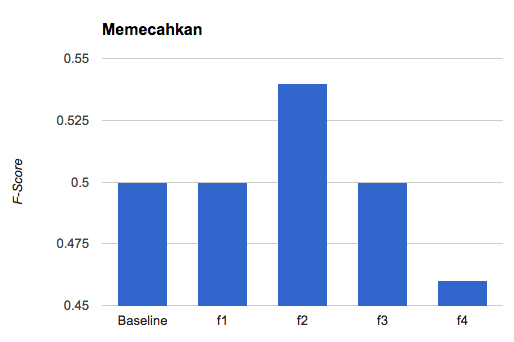
\includegraphics[width=1\linewidth]{adit_pics/memecahkan.png}
		\caption{memecahkan}
	\end{subfigure}%
	\begin{subfigure}{.5\textwidth}
		\centering
		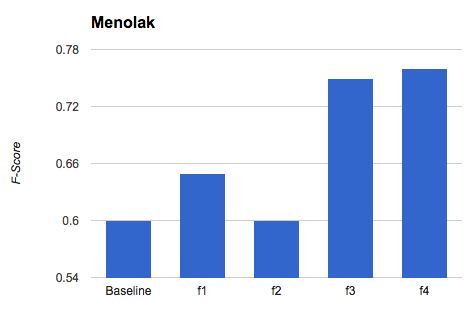
\includegraphics[width=1\linewidth]{adit_pics/menolak.png}
		\caption{menolak}
	\end{subfigure}%
	\\
	\begin{subfigure}{.5\textwidth}
		\centering
		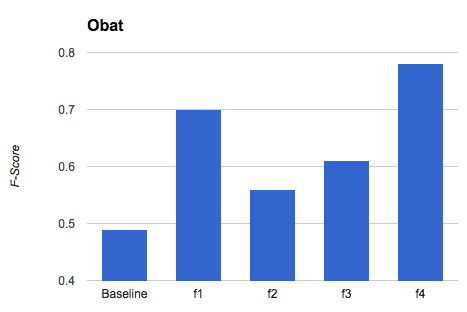
\includegraphics[width=1\linewidth]{adit_pics/obat.png}
		\caption{obat}
	\end{subfigure}%
	\begin{subfigure}{.5\textwidth}
		\centering
		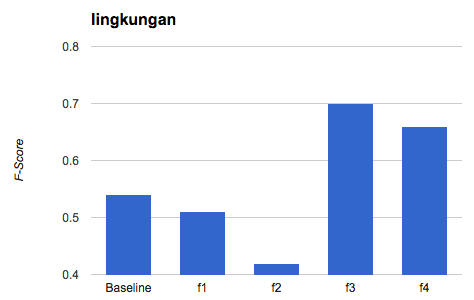
\includegraphics[width=1\linewidth]{adit_pics/lingkungan.png}
		\caption{lingkungan}
	\end{subfigure}%
	\\
	\begin{subfigure}{.5\textwidth}
		\centering
		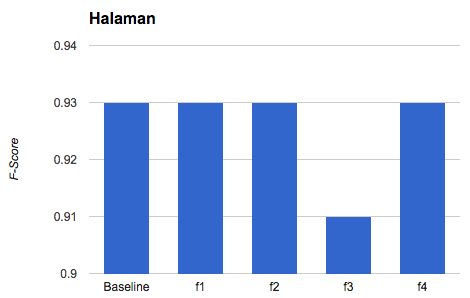
\includegraphics[width=1\linewidth]{adit_pics/halaman.png}
		\caption{halaman}
	\end{subfigure}%
	\begin{subfigure}{.5\textwidth}
		\centering
		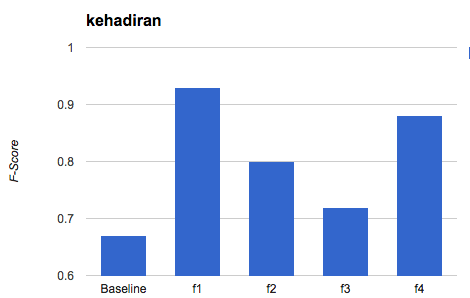
\includegraphics[width=1\linewidth]{adit_pics/kehadiran.png}
		\caption{kehadiran}
	\end{subfigure}%
	\\
	\begin{subfigure}{.5\textwidth}
		\centering
		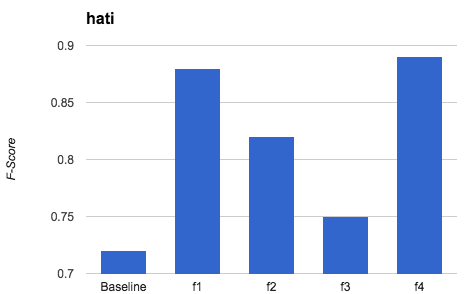
\includegraphics[width=1\linewidth]{adit_pics/hati.png}
		\caption{hati}
	\end{subfigure}%
	\begin{subfigure}{.5\textwidth}
		\centering
		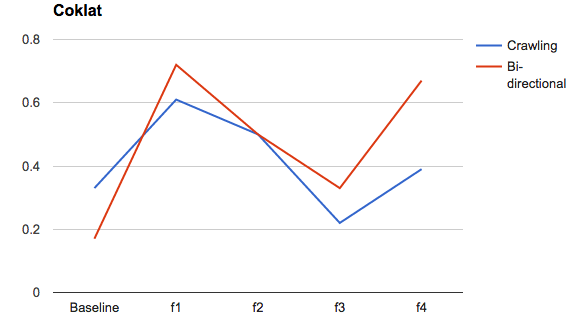
\includegraphics[width=1\linewidth]{adit_pics/coklat.png}
		\caption{coklat}
	\end{subfigure}%
\end{figure}
\clearpage	
\begin{figure}[H]
	\ContinuedFloat
	\begin{subfigure}{.5\textwidth}
		\centering
		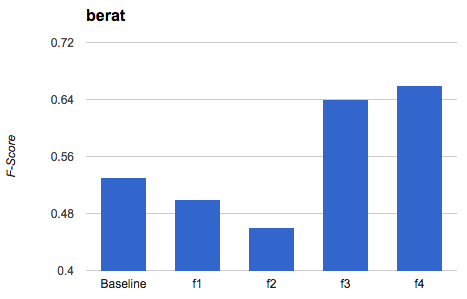
\includegraphics[width=1\linewidth]{adit_pics/berat.png}
		\caption{berat}
	\end{subfigure}%
	\begin{subfigure}{.5\textwidth}
		\centering
		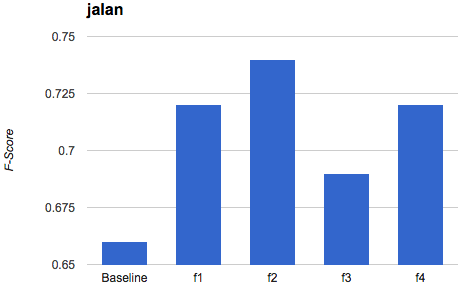
\includegraphics[width=1\linewidth]{adit_pics/jalan.png}
		\caption{jalan}
	\end{subfigure}%
	\caption{Grafik Performa Fitur WSD Bahasa Indonesia}
	\label{fig:fitur-wsd-indo}
\end{figure} 

Berdasarkan sepuluh grafik di atas, dapat kita lihat bahwa sembilan dari sepuluh \textit{sample} kata yang dicoba, hanya satu kata yang tidak pernah memiliki performa lebih baik baseline yaitu kata "halaman". Sembilan kata lainnya selalu memiliki performa di atas baseline untuk minimal satu dari keempat fitur yang dicoba. Pada tujuh buah \textit{sample}, fitur F2 memiliki akurasi di bawah F1 walaupun sudah menggunakan \textit{word embedding}. Pada lima buah \textit{sample} kata, F4 yang merupakan fitur gabungan F1 dan F3 memiliki performa yang lebih baik dari fitur F1 saja. Penggunaan berbagai skenario fitur tersebut menunjukan bahwa fitur F1 atau F4 memiliki performa minimal sama atau di atas baseline pada sembilan dari sepuluh \textit{sample} (90\%), hal ini menunjukkan bahwa \textit{bag of words} ataupun kombinasinya dengan POS Tag dapat mengungguli baseline pada \textit{sampling} ini. Jumlah persentase pada \textit{sampling} dengan fitur F2 yang mengungguli baseline adalah 70\%. Performa F2 yang lebih rendah dari F4 pada rerata F-Score dapat disebabkan karena domain yang berbeda antara \textit{training data} pada saat membentuk model \textit{word embedding} (perbedaan pada gaya bahasa pada Wikipedia dan korpus identik). Namun demikian, persentase terbesar dari \textit{sampling} sepuluh kata di atas diperoleh pada fitur F4 yang memiliki performa lebih baik dari baseline pada sembilan kasus dari sepuluh kata tersebut (90\%).
%!TEX root = skripsi.tex
%-----------------------------------------------------------------------------%
\chapter{\babEnam}
%-----------------------------------------------------------------------------%

%-----------------------------------------------------------------------------%
\section{Kesimpulan}
%-----------------------------------------------------------------------------%

Data dan \textit{resource} berupa \textit{sense tagged corpus} yang terbatas pada bahasa Indonesia merupakan penghambat dari penelitian WSD di Bahasa Indonesia. Untuk mengatasi masalah tersebut, salah satu pendekatan WSI berupa \textit{cross lingual} dapat dimanfaatkan untuk \textit{transfering knowledge} dari salah satu bahasa dengan data yang lebih banyak yaitu bahasa Inggris.

Konsep pendekatan \textit{cross lingual sense transfering} ini dapat menghasilkan \textit{sense tagged corpus} bahasa Indonesia dengan memindahkan makna kata dari korpus bahasa Inggris ke kata-kata yang menjadi pasangannya (\textit{translation} dari kata tersebut) di dalam Bahasa Indonesia. Metode yang digunakan untuk membangun \textit{sense tagged corpus} tersebut meliputi \textit{tagging} pada korpus Bahasa Inggris dengan menggunakan \textit{tool} IMS \citep{zhong2010makes}, melakukan \textit{alignment} kata pada korpus identik (Inggris-Indonesia) dengan Giza++ \citep{och03:asc}, dan \textit{sense transfering} untuk memindahkan makna kata tersebut. \textit{Sense tagged corpus} Bahasa Indonesia  yang merupakan hasil dari proses tersebut memiliki kualitas cukup baik walaupun masih terdapat makna kata yang tidak tepat karena kesalahan pada proses \textit{tagging} korpus bahasa Inggris ataupun \textit{alignment}.

Pada penelitian yang dilakukan, sistem WSD dibuat dengan \textit{classifier} SVM dan dicoba dengan empat skenario fitur, yaitu \textit{bag of words} (F1), \textit{word embedding} (F2), POS Tag (F3), dan gabungan antara F1 dengan F3 (F4). Sistem tersebut  memiliki performa yang lebih baik dari baseline pada kebanyakan kasus untuk fitur tertentu. Fitur dengan persentase terbaik pada penelitian ini adalah gabungan dari fitur \textit{bag of words} dan POS Tag yang mengungguli baseline pada 80\% \textit{sample} kata percobaan dengan nilai rerata F-Score terbesar yaitu 68.2\%.
%-----------------------------------------------------------------------------%
\section{Saran}
%-----------------------------------------------------------------------------%
Setelah melakukan percobaan dan melakukan analisis hasil dari penelitian ini, terdapat beberapa saran untuk penelitian selanjutnya diantaranya sebagai berikut.

\begin{enumerate}
	\item Penggunaan kualitas dari korpus paralel dapat mempengaruhi seberapa baik hasil \textit{sense transfering} yang dilakukan. Pada korpus identik yang penelitian ini gunakan dengan jumlah kalimat sebanyak 88.919 buah, terdapat beberapa kalimat yang terpotong maupun \textit{comparable} (tidak sepenuhnya paralel), sehingga rawan menimbulkan kesalahan \textit{alignment}.
	\item \textit{Transferring} makna kata yang dilakukan mungkin dapat dibantu juga dengan informasi POS Tag ataupun \textit{word embedding}. Pada informasi POS Tag, makna kata yang dipindahkan mungkin dapat diperiksa kesamaan antara POS Tag yang dimilikinya dengan \textit{sense key} yang akan dipindahkan. Informasi vektor dari \textit{word embedding} sendiri juga mungkin dapat digunakan dengan mengubah representasi \textit{sense} dengan \textit{word embedding}, namun hal ini akan memerlukan penelitian yang lebih dalam lagi.
	\item Fitur yang digunakan dalam sistem WSD bahasa Indonesia masih dapat ditambahkan dengan berbagai fitur lainnya seperti Collocation, \textit{text rank}, \textit{dependancy parser}, dan lain-lain.
	\item \textit{Classifier} pada sistem WSD juga dapat diganti dengan yang lain seperti misalnya Naive Bayes, Multilayer Perceptron, dan lain-lain. Arsitektur juga dapat dicoba untuk menggunakan pendekatan \textit{deep learning} pada penelitian selanjutnya.
	\item Proses \textit{word alignment} sebaiknya dilakukan dengan \textit{tool} SMT yang mempunyai model lebih baru seperti misalnya berkeley aligner. Selain \textit{tool}, teknik hybrid seperti misalnya menggabungkan \textit{alignment} dari \textit{tool} yang berbeda juga mungkin dapat dicoba untuk meningkatkan kualitas dari \textit{word alignment} yang dihasilkan.
\end{enumerate}

%\printbibliography
%
% Daftar Pustaka
%\include{pustaka}
%biblama (bukan biblatex)
\bibliography{skripsi}{}
%\bibliography{references}{}
%biblama (bukan biblatex)
\bibliographystyle{apalikerd}
%\bibliographystyle{ieeetr} 

%
% Lampiran 
%
% \begin{appendix}
% 	%!TEX root = skripsi.tex
%
% @author  Andreas Febrian
% @version 1.00 
% 
% Hanya sebuah pembatas bertuliskan LAMPIRAN ditengah halaman. 
% 

\begin{titlepage}
	\centering 
	\vspace*{6cm}
	\noindent \Huge{LAMPIRAN}
	\addChapter{LAMPIRAN}
\end{titlepage}
% 	\setcounter{page}{2}
% 	%!TEX root = skripsi.tex

\addChapter{Lampiran 1 : Panduan Evaluasi \textit{Word Alignment}}

%\chapter*{Lampiran 1 : Panduan Evaluasi \textit{Word Alignment}}

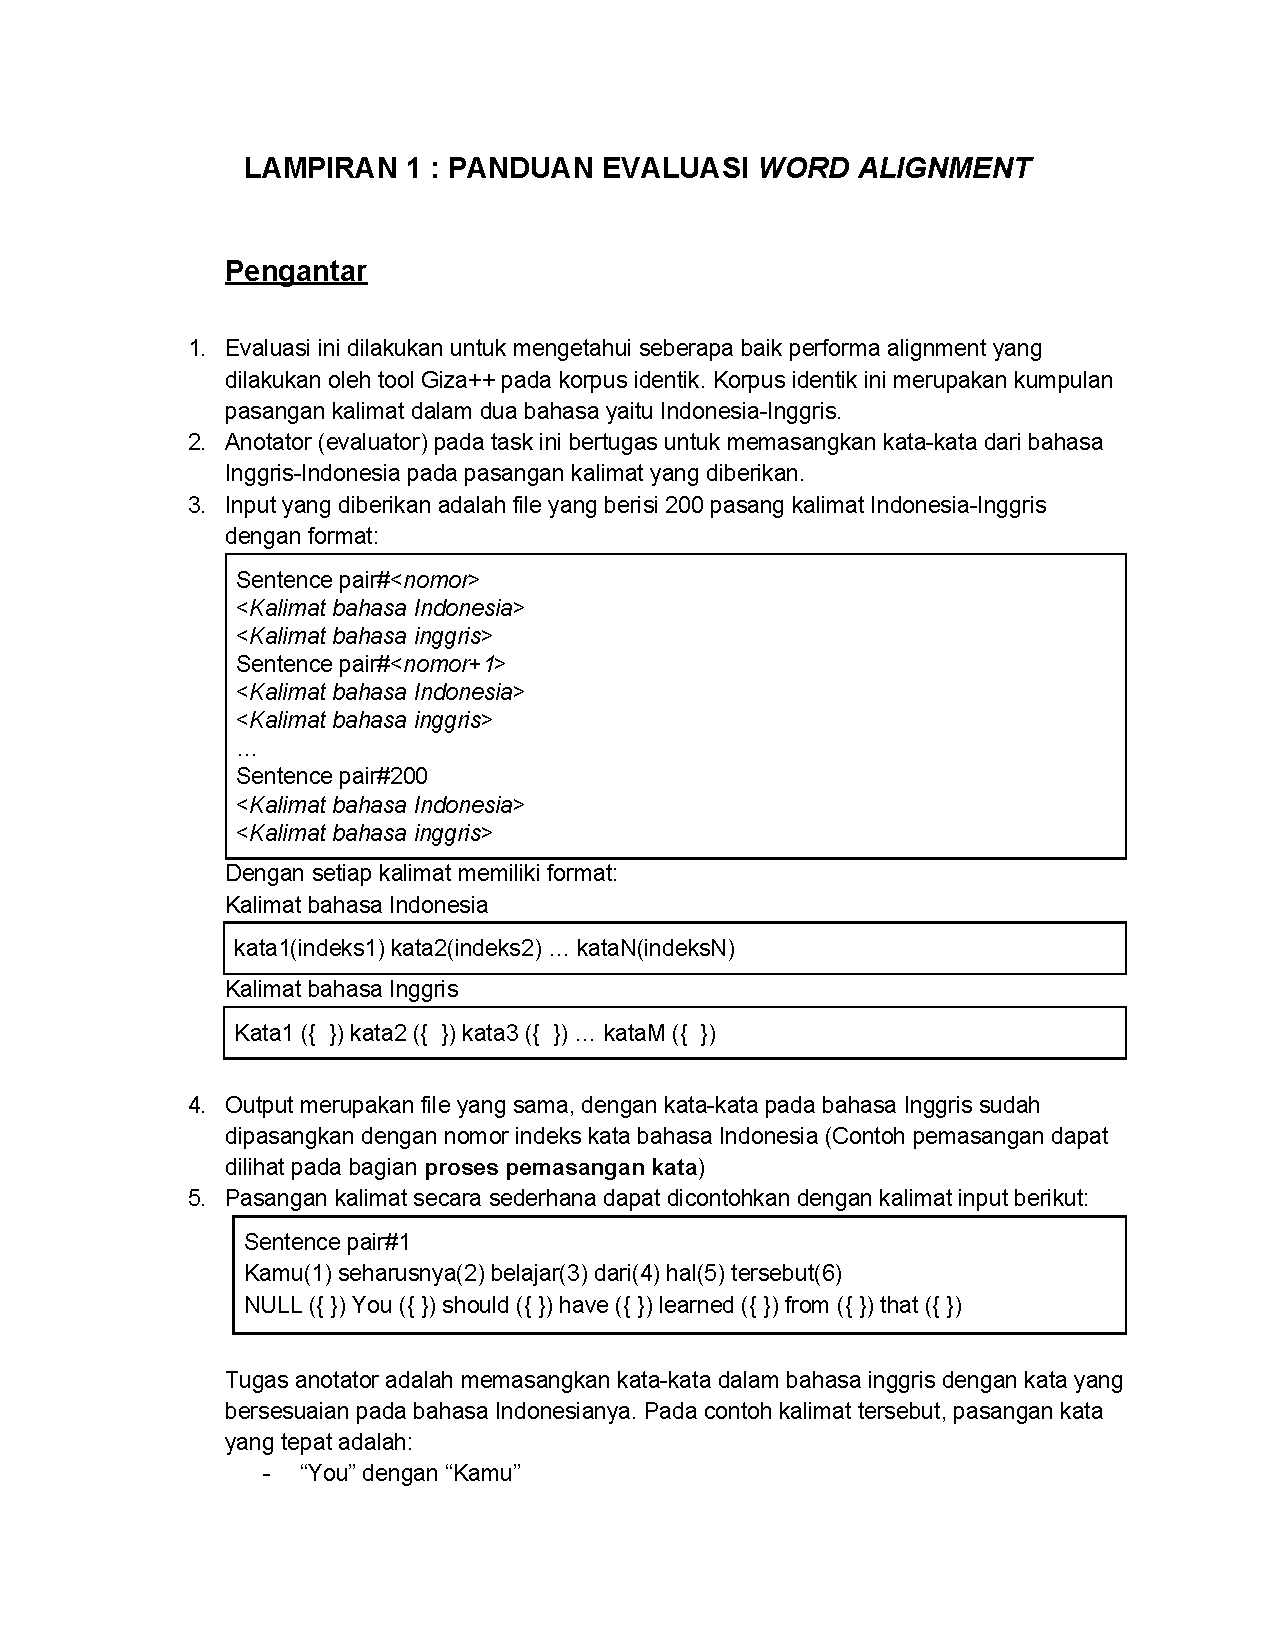
\includepdf[pages={-}, pagecommand={}]{pewa_1.pdf}

\begin{comment}


\section*{Pengantar}

\begin{enumerate}
	\item Evaluasi ini dilakukan untuk mengetahui seberapa baik performa alignment yang dilakukan oleh tool Giza++ pada korpus identik. Korpus identik ini merupakan kumpulan pasangan kalimat dalam dua bahasa yaitu Indonesia-Inggris.
	\item Anotator (evaluator) pada task ini bertugas untuk memasangkan kata-kata dari bahasa Inggris-Indonesia pada pasangan kalimat yang diberikan.
	\item Input yang diberikan adalah file yang berisi 200 pasang kalimat Indonesia-Inggris dengan format:
\begin{lstlisting}[backgroundcolor = \color{white}]
Sentence pair#< nomor >
< Kalimat bahasa Indonesia >
< Kalimat bahasa Indonesia >
Sentence pair#< nomor+1 >
< Kalimat bahasa Indonesia >
< Kalimat bahasa inggris >
...
Sentence pair#200
< Kalimat bahasa Indonesia >
< Kalimat bahasa inggris >
\end{lstlisting}
	Dengan setiap kalimat memiliki format:\\
	Kalimat bahasa Indonesia
\begin{lstlisting}[backgroundcolor = \color{white}]
kata1(indeks1) kata2(indeks2) ... kataN(indeksN)
\end{lstlisting}	
Kalimat bahasa Inggris
\begin{lstlisting}[backgroundcolor = \color{white}]
Kata1 ({ }) kata2 ({ }) kata3 ({ }) ... kataM ({ })
\end{lstlisting}
	\item Output merupakan file yang sama, dengan kata-kata pada bahasa Inggris sudah dipasangkan dengan nomor indeks kata bahasa Indonesia (Contoh pemasangan dapat dilihat pada bagian \textbf{proses pemasangan kata})
	\item Pasangan kalimat secara sederhana dapat dicontohkan dengan kalimat input berikut:
\begin{lstlisting}[backgroundcolor = \color{white}]
Sentence pair#1
Kamu(1) seharusnya(2) belajar(3) dari(4) hal(5) tersebut(6)
Kamu(1) seharusnya(2) belajar(3) dari(4) hal(5) tersebut(6)
\end{lstlisting}
	Tugas anotator adalah memasangkan kata-kata dalam bahasa inggris dengan kata yang bersesuaian pada bahasa Indonesianya. Pada contoh kalimat tersebut, pasangan kata yang tepat adalah:
	\begin{enumerate}
		\item 'You' dengan 'kamu'
		\item 'should' dengan 'seharusnya'
		\item 'learned' dengan 'belajar'
		\item 'from' dengan 'dari'
		\item 'that' dengan 'hal tersebut'
	\end{enumerate}
\end{enumerate}

\section*{Proses Pemasangan Kata}
\begin{enumerate}
	\item Diberikan pasangan kalimat dalam bahasa Inggris dan bahasa Indonesia sebanyak 200 buah pasangan:\\
	contoh \textbf{input} pasangan 1:
	
\end{enumerate}

\end{comment}
% \end{appendix}

%!TEX root = skripsi.tex

\addChapter{Lampiran 1 : Panduan Evaluasi \textit{Word Alignment}}

%\chapter*{Lampiran 1 : Panduan Evaluasi \textit{Word Alignment}}

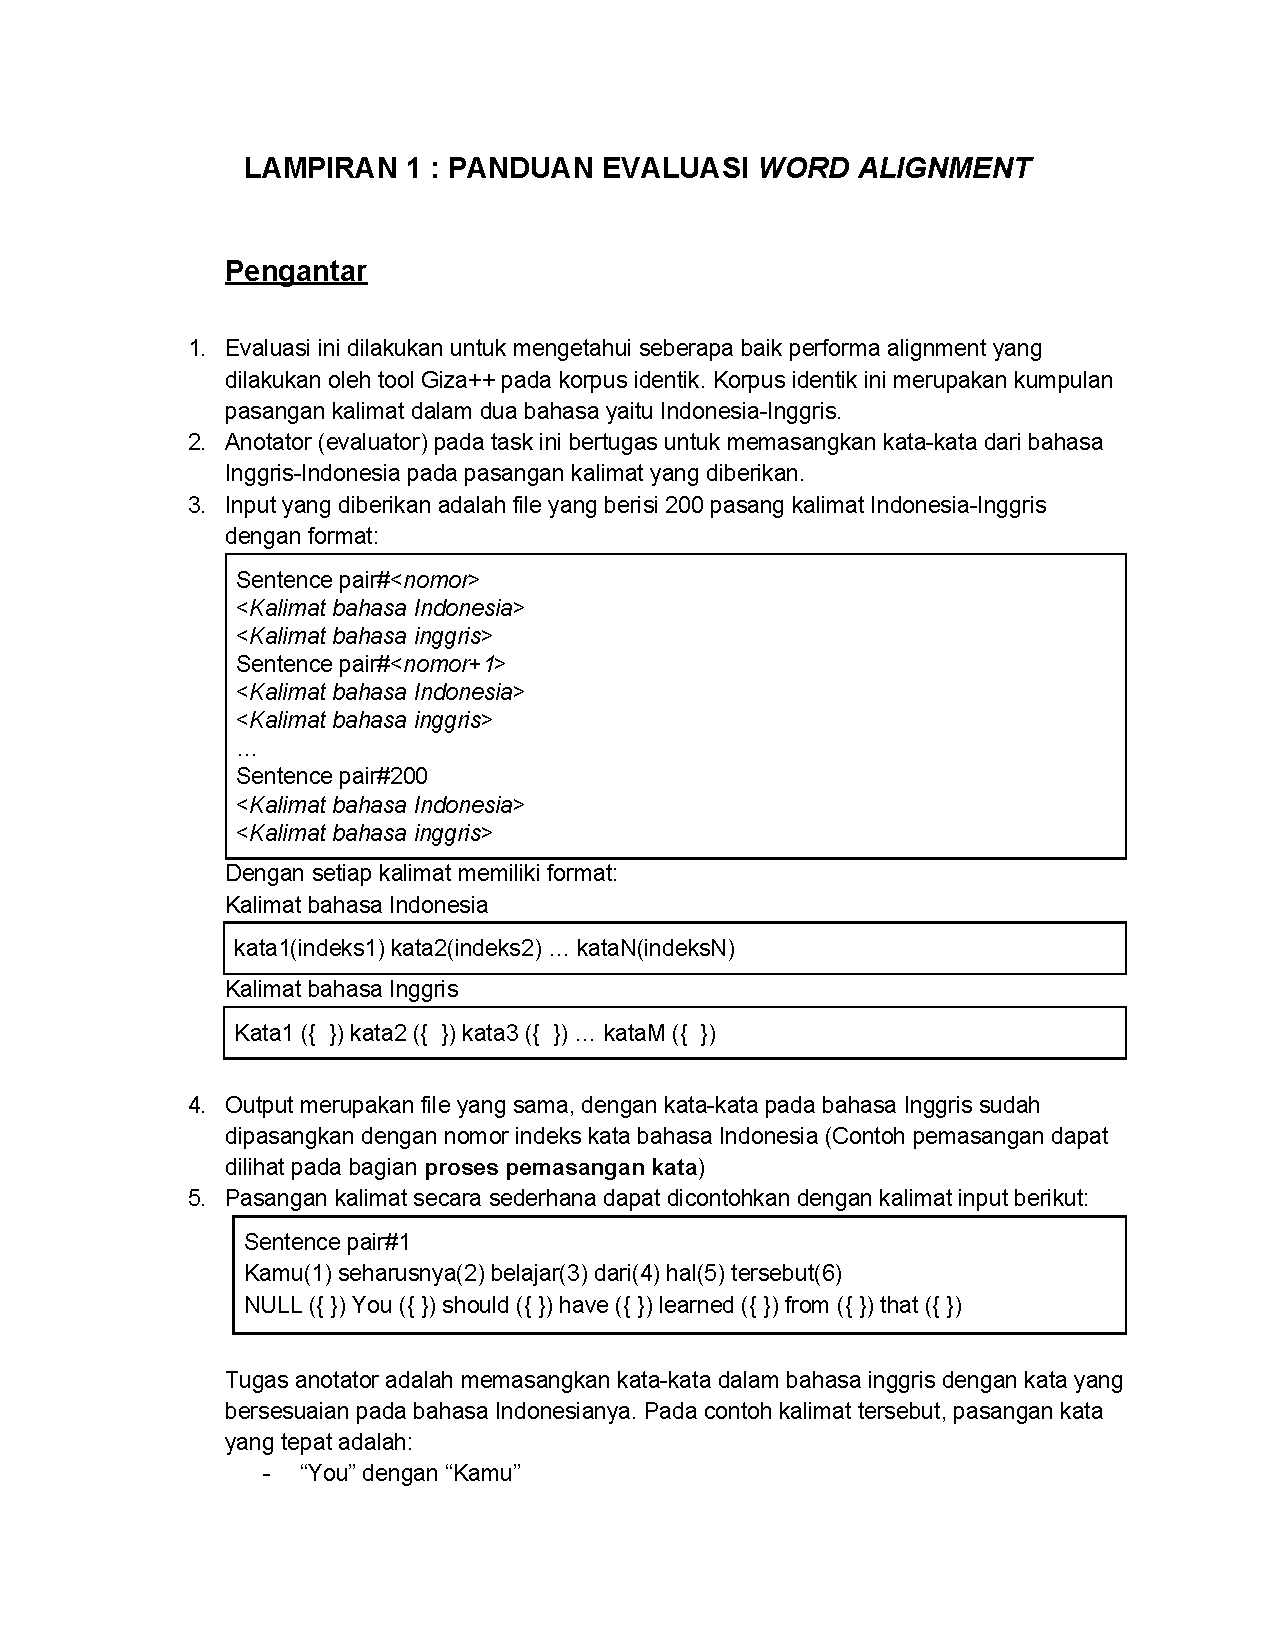
\includepdf[pages={-}, pagecommand={}]{pewa_1.pdf}

\begin{comment}


\section*{Pengantar}

\begin{enumerate}
	\item Evaluasi ini dilakukan untuk mengetahui seberapa baik performa alignment yang dilakukan oleh tool Giza++ pada korpus identik. Korpus identik ini merupakan kumpulan pasangan kalimat dalam dua bahasa yaitu Indonesia-Inggris.
	\item Anotator (evaluator) pada task ini bertugas untuk memasangkan kata-kata dari bahasa Inggris-Indonesia pada pasangan kalimat yang diberikan.
	\item Input yang diberikan adalah file yang berisi 200 pasang kalimat Indonesia-Inggris dengan format:
\begin{lstlisting}[backgroundcolor = \color{white}]
Sentence pair#< nomor >
< Kalimat bahasa Indonesia >
< Kalimat bahasa Indonesia >
Sentence pair#< nomor+1 >
< Kalimat bahasa Indonesia >
< Kalimat bahasa inggris >
...
Sentence pair#200
< Kalimat bahasa Indonesia >
< Kalimat bahasa inggris >
\end{lstlisting}
	Dengan setiap kalimat memiliki format:\\
	Kalimat bahasa Indonesia
\begin{lstlisting}[backgroundcolor = \color{white}]
kata1(indeks1) kata2(indeks2) ... kataN(indeksN)
\end{lstlisting}	
Kalimat bahasa Inggris
\begin{lstlisting}[backgroundcolor = \color{white}]
Kata1 ({ }) kata2 ({ }) kata3 ({ }) ... kataM ({ })
\end{lstlisting}
	\item Output merupakan file yang sama, dengan kata-kata pada bahasa Inggris sudah dipasangkan dengan nomor indeks kata bahasa Indonesia (Contoh pemasangan dapat dilihat pada bagian \textbf{proses pemasangan kata})
	\item Pasangan kalimat secara sederhana dapat dicontohkan dengan kalimat input berikut:
\begin{lstlisting}[backgroundcolor = \color{white}]
Sentence pair#1
Kamu(1) seharusnya(2) belajar(3) dari(4) hal(5) tersebut(6)
Kamu(1) seharusnya(2) belajar(3) dari(4) hal(5) tersebut(6)
\end{lstlisting}
	Tugas anotator adalah memasangkan kata-kata dalam bahasa inggris dengan kata yang bersesuaian pada bahasa Indonesianya. Pada contoh kalimat tersebut, pasangan kata yang tepat adalah:
	\begin{enumerate}
		\item 'You' dengan 'kamu'
		\item 'should' dengan 'seharusnya'
		\item 'learned' dengan 'belajar'
		\item 'from' dengan 'dari'
		\item 'that' dengan 'hal tersebut'
	\end{enumerate}
\end{enumerate}

\section*{Proses Pemasangan Kata}
\begin{enumerate}
	\item Diberikan pasangan kalimat dalam bahasa Inggris dan bahasa Indonesia sebanyak 200 buah pasangan:\\
	contoh \textbf{input} pasangan 1:
	
\end{enumerate}

\end{comment}

\end{document}